\documentclass{article}

\usepackage[english]{babel}
\usepackage{amsmath}
\usepackage{amssymb}
\usepackage{amsthm}
\usepackage[font=small]{caption}
\usepackage{cite}
\usepackage{graphicx}

\newtheorem{algorithm}{Algorithm}
\newtheorem{definition}{Definition}
\newtheorem{example}{Example}
\newtheorem{lemma}{Lemma}
\newtheorem{proposition}{Proposition}
\newtheorem{remark}{Remark}

%---------------------------------------------------------------

\title{Analytic combinatorics meets bioinformatics I: applications to
seeding methods}
\author{
\textsc{Guillaume Filion and Eduard Valera Zorita} \\ [1ex]
\normalsize CRG, Barcelona
}
\date{\today}

%---------------------------------------------------------------
%---------------------------------------------------------------


\begin{document}

\maketitle

\begin{abstract}
The abstract will come later.
\end{abstract}


%---------------------------------------------------------------
%---------------------------------------------------------------

\section{Introduction}

High throughput sequencing is changing the face of biology. More data is
of course better, but recently, technical improvements have started to
outpace the progress of algorithms. When the problems are too large,
one has to replace exact algorithms by heuristics that are much faster,
but do not guarantee to return the right result. Good heuristics are all
about understanding the input data. With the right model of the data, we
can calculate the risk of not returning the right answer and adjust the
algorithm to achieve more precision or more speed. When the data is poorly
understood, heuristics may be slow or inefficient for unknown reasons.

A particular area of bioinformatics where heuristics have been in use for
a long time is the field of sequence alignment. Computing the best
alignment between two sequences is carried out by dynamic programming in
time $O(mn)$, where $m$ and $n$ are the sequence lengths. When at least
one of the sequences is long (\textit{e.g.} a genome), this is prohibitive
and heuristics are required.

The most studied heuristics for sequence alignment are called seeding
methods. In a nutshell, the idea is to search short regions of the two
sequences that are very similar and use them as candidates to anchor the
dynamic programming alignment, which is performed only locally
\textit{i.e.} between subsequences of the input. These short regions of
high similarity are called ``seeds''. The benefit of the approach is that
seeds can be found in short time. The risk is that they may not exist,
even if the input sequences are similar.

This strategy was most famously implemented in BLAST for the purpose of
finding local homology between proteins. By working out an approximate
distribution of the identity score for the seeds, the authors were able to
calibrate the BLAST heuristic very accurately in order to gain speed. The
algorithm always performs the minimum amount of work for a desired
confidence level (acceptable false negative rate).

Seeding methods are also heavily used in the mapping problem, where the
original sequence of a read must be found in a reference genome. The
dicovery of indexing methods based on the Burrows-Wheeler transform was
instrumental to develop short read mappers such as BWA and Bowtie. With
such indexes, one can know the number of occurrences of a substring in a
genome in time independent of the genome size. This yields an obvious
seeding strategy whereby all the substrings of the read are queried in the
genome. Here the seeds must have exactly the same sequence in the read and
in the genome.

The heuristic should be calibrated from the probability that a seed of
given length can be found in the read, but this problem has not been fully
solved. The answer depends on the types and frequencies of errors, which
are often context-dependent. Overall, the lack of theoretical framework to
model seeding probabilities is halting progress on this line of research.

Here we solve this problem for abitrary error models using the powerful
theory of analytic combinatorics. This field of research was initiated by
Donlad Knuth in the early days of algorithmics, and later developed by
Robert Sedgewick and Philippe Flajolet. The theory is now mature and used
to tackle may problems outside the analysis of algorithms. However, it
has not yet been realized how useful it can be for bioinformatics.

This document is predominantly written for bioinformaticians and people
with a working knowledge of sequencing technologies and their applications.
Accordingly, the focus will be on explaining the mathematical concepts,
rather than the technological aspects. Also, our goal here is not to push
the boundaries of analytic combinatorics, but to explain how its simplest
concepts are useful to solve common problems in bioinformatics. We have
opted for simplicity, to the detriment of generality and rigor. The
results presented here are only a basic introduction to analytic
combinatorics; the field is currently much more advanced and we refer the
interested to the original literature.

\section{Analytic combinatorics}
\label{sec:anal}

\subsection{Weighted generating functions}
\label{subsec:WGF}

\begin{definition}
\label{def:GF}
Let $\mathcal{A}$ be a set of combinatorial objects characterized by a
size and a weight. The \textbf{weighted generating function} of
$\mathcal{A}$ is defined as

\begin{equation}
\label{eq:GF1}
A(z) = \sum_{a \in A} w(a) z^{|a|},
\end{equation}

\noindent
where $|a|$ and $w(a)$ denote the size and weight of the object $a$,
respectively. This also defines a sequence $(a_k)_{k \geq 0}$ such that 

\begin{equation}
\label{eq:GF2}
A(z) = \sum_{k=0}^\infty a_k z^k.
\end{equation}

By definition $a_k = \sum_{a \in A_k}w(a)$, where $A_k$ is the class of
objects of size $k$. The number $a_k$ is called the total weight of
objects of size $k$.
\end{definition}

\begin{remark}
\label{rem:noweight}
If the weight of every object $a \in \mathcal{A}$ is $1$, then $A(z)$ is a
simple generating function and $a_k$ in expression (\ref{eq:GF2}) is
the number of objects of size $k$.
\end{remark}

Note that in definition \ref{def:GF}, the weight is a property of
combinatorial objects and the total weight is a property of a classes of
ojects. Expressions (\ref{eq:GF1}) and (\ref{eq:GF2}) are equivalent.
Depending on the context, we will use one or the other.

The essence of analytic combinatorics is that some operations on
combinatorial objects correspond to some operations on their generatintg
function. If $A(z)$ and $B(Z)$ are the weighted generating functions of
two mutually exclusive sets $\mathcal{A}$ and $\mathcal{B}$, the weighted
generating function of $\mathcal{A} \cup \mathcal{B}$ is $A(z) + B(z)$, as
appears immediately from expression (\ref{eq:GF1}). Size and weight can be
extended to pairs of objects in $\mathcal{A} \times \mathcal{B}$ by
defining $|(a,b)| = |a| + |b|$ and $w(a,b) = w(a)w(b)$. With this
convention, the weighted generating function of $\mathcal{A} \times
\mathcal{B}$ is $A(z)B(z)$, as shown by expression (\ref{eq:GF1})
once again

\begin{equation*}
A(z)B(z) =
\sum_{a\in \mathcal{A}}w(a)z^{|a|} \sum_{b\in \mathcal{B}}w(b)z^{|b|}
= \sum_{(a,b) \in \mathcal{A} \times \mathcal{B}} w(a)w(b)z^{|a|+|b|}.
\end{equation*}

\begin{example}
\label{ex:simple}
Assume that $\mathcal{A}$ contains a single object $a$ of size $1$ and of
weight $p$. The weighted generating function of $\mathcal{A}$ is $pz$.
The set $\mathcal{A}^2$ contains a single object $(a,a)$ of size $2$ and
weight $p^2$. Its weighted generating function is $p^2z^2 = pz \cdot pz$.
\end{example}

The definition of size and weight can be further extended to any finite
Cartesian product in the same way. The generating function of a cartesian
product then comes as the product of their generating functions.

\begin{example}
\label{ex:sequences}
Following up on example~\ref{ex:simple}, the set $\mathcal{A}^k$ contains
a single object of size $k$ and weight $p^k$, and its weighted generating
function is $p^kz^k$. Since the sets $\mathcal{A}, \mathcal{A}^2,
\mathcal{A}^3,\ldots$ are mutually exclusive, the weighted generating
function of their union is

\begin{equation*}
pz + (pz)^2 + (pz)^3 \ldots
\end{equation*}

For any given $k$, notice that $(1-pz) \big(pz + (pz)^2 + \ldots + (pz)^k
\big) = pz-(pz)^{k+1}$.  If $|z| < 1/p$, the term $(pz)^{k+1}$ vanishes as
$k$ increases. So the weighted generating function is defined for $|z| <
1/p$ and is equal to

\begin{equation*}
pz + (pz)^2 + (pz)^3 \ldots = \frac{pz}{1-pz}.
\end{equation*}
\end{example}

Example~\ref{ex:sequences} can be generalized. For any set $\mathcal{A}$,
objects of $\mathcal{A}^+ = \cup_{k=1}^\infty\mathcal{A}^k$ are called
nonempty (finite) sequences of objects of $\mathcal{A}$. By defining
$\mathcal{A}^0$ as the set containg only $\varepsilon$, the ``empty''
object of size 0 and weight 1, we can also define $\mathcal{A}^* =
\cup_{k=0}^\infty\mathcal{A}^k$ as the set of sequences of objects of
$\mathcal{A}$.

\begin{proposition}
\label{th:sequences}
Let $\mathcal{A}$ be a set with weighted generating function $A(z)$. The
generating functions of $\mathcal{A}^+$ and $\mathcal{A}^*$ are defined
for $|A(z)| < 1$ and are respectively equal to

\begin{equation*}
\begin{split}
\frac{A(z)}{1-A(z)}&\text{, and} \\
\frac{1}{1-A(z)}&.
\end{split}
\end{equation*}
\end{proposition}

\begin{proof}
For $k \geq 1$, the generating function of $\mathcal{A}^k$ is $A(z)^k$ and
since the sets are mutually exclusive, the weighted generating function of
their union $\mathcal{A}^+$ is $A(z) + A(z)^2 + \ldots = A(z) / (1-A(z))$,
provided $|A(z)| < 1$.

The generating function of $\mathcal{A}^0$ is $1$ so the weighted
generating function of $\mathcal{A}^*$ is $1 + A(z) + A(z)^2 + \ldots =
1 / (1-A(z))$, provided $|A(z)| < 1$.
\end{proof}

\begin{remark}
These expressions are not defined for $A(z) = 1$, \textit{i.e.} when
$\mathcal{A}$ contains only the empty object. In other words, one cannot
construct sequences of empty ojects.
\end{remark}

From here on, we will not state the conditions of definition of the
generating functions. We will simply assume that $|z|$ is lower than the
radius of convergence of the given expression.

Let us illustrate how to count with generating functions. Following
remark~\ref{rem:noweight}, if the weights of all the objects are equal to
$1$, then the coefficient of $z^k$ in (\ref{eq:GF2}) is the number of
objects of size $k$.

\begin{example}
\label{ex:noweight}
Let $\mathcal{A}$ and $\mathcal{B}$ be alphabets with only one symbol
each. Say $\mathcal{A} = \{a\}$ and $\mathcal{B} = \{b\}$. Each symbol
has weight $1$, so the simple generating function of each alphabet is $z$.
The generating function of $\mathcal{A} \cup \mathcal{B}$, the alphabet
with both symbols is $z+z = 2z$. This means that $\mathcal{A} \cup
\mathcal{B}$ contains two objects of size $1$ and nothing else.

Let us now combine the symbols into sequences and count them. By
proposition~\ref{th:sequences}, the generating function of sequences of
letters from $\mathcal{A} \cup \mathcal{B}$ is

\begin{equation*}
\frac{1}{1-2z} = 1 + 2z + (2z)^2 + (2z)^3 + \ldots
\end{equation*}

The coefficient of $z^k$ in this expression is $2^k$. In other words,
there are $2^k$ sequences of size $k$ made of the two symbols $a$ and $b$.
\end{example}

If some objects are more frequent or more common than others, we can give
them different weights. Let us revisit the previous example with a slight
modification.

\begin{example}
\label{ex:wweights}
Assume once again that $\mathcal{A} = \{a\}$ and $\mathcal{B} = \{b\}$,
but this time $a$ has frequency $1/3$ and $b$ has frequency $2/3$. The
weighted generating function of $\mathcal{A}$ is $z/3$ and that of
$\mathcal{B}$ is $2z/3$. The generating function of $\mathcal{A} \cup
\mathcal{B}$ is $z/3 + 2z/3 = z$. This does not say how many objects are
in $\mathcal{A} \cup \mathcal{B}$ but it says that there only objects of
size $1$ and that their total weight is $1$.

As in example~\ref{ex:noweight}, let us combine the symbols into
sequences. The generating function of sequences of letters from
$\mathcal{A} \cup \mathcal{B}$ is

\begin{equation*}
\frac{1}{1-z} = 1 + z + z^2 + z^3 + \ldots
\end{equation*}

For every $k \geq 0$, the coefficient of $z^k$ in this expression is $1$,
so there are sequences of all sizes. This does not give the number of
sequences of each size, but it says that their total weight is $1$.

This may seem useless, but let us now evaluate the probatility that a
sequence does not contain any $b$. In that case, it is a sequence of
elements of $\mathcal{A}$, of which the weighted generating function is

\begin{equation*}
\frac{1}{1-z/3} = 1 + z/3 + (z/3)^2 + (z/3)^3 + \ldots
\end{equation*}

The coefficient of $z^k$ is $1/3^k$ so sequences of size $k$ that contain
no $b$ have a total weight equal to $1/3^k$. Since the total weight of
sequences of size $k$ is $1$, the total weight of sequences that do not
contain any $b$ is $1/3^k \big/ 1 = 1/3^k$.
\end{example}

In example~\ref{ex:wweights}, the weighted generating function of the
sequence $aaaba$ is $z/3 \times z/3 \times z/3 \times 2z/3 \times z/3 =
2z^5/243$, which is another way of saying that $aaaba$ has size $5$ and
weight $2/243$. Observe that if the symbols are chosen independently of
each other, $2/243$ is the probability that a sequence of size $5$ is
equal to $aaaba$. This is a general feature of weights. In the
applications below, they will always be equal to the probability
of occurrence of the objects they mark.

The coefficients of weighted generating functions expressed as in
(\ref{eq:GF2}) thus represent the probabilities of occurrence of some
objects of interest. This observation motivates the search for
their weighted generating function.



%%%%%%%%%%%%%%%%% Transfer matrices %%%%%%%%%%%%%%%%%

\subsection{Sequences and transfer matrices}

In many combinatorial applications, one needs to count the sequences where
a pattern does or does not occur. A convenient way to find the weighted
generating functions of such sequences is to use transfer matrices in
order to encode the allowed or disallowed patterns. We will illustrate
the process informally with an example from biology, before introducing
the formal definitions.

DNA methylation can only occur on the dinucleotide \texttt{CG}s in many
animal genomes. Because of this property, it is interesting to count the
sequences that have no \texttt{CG}. Such a sequence is a walk on the
graph with restricted transitions shown in figure~\ref{fig:CG_transtions}.

\begin{figure}[h]
\centering
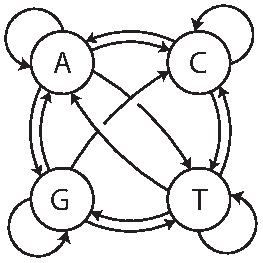
\includegraphics[scale=0.9]{CG_transitions.pdf}
\caption{\textbf{Graph with restricted transitions}.
A sequence without \texttt{CG} can be seen as a walk on the graph above.
All the transitions are allowed, except \texttt{C} to \texttt{G}.}
\label{fig:CG_transtions}
\end{figure}

Arranging the nodes in alphabetical order, the adjacency matrix of the
directed graph is

\begin{equation*}
M = \left[
\begin{matrix}
1 & 1 & 1 & 1 \\
1 & 1 & 0 & 1 \\
1 & 1 & 1 & 1 \\
1 & 1 & 1 & 1
\end{matrix}
\right].
\end{equation*}

The entry of the matrix $M^n$ at position $(i,j)$ corresponds to the
number of paths on this graph that start with nucleotide $i$, end with
nucleotide $j$ and contain $n$ steps. So a way to count sequences without
\texttt{CG} is to compute the powers of the adjacency matrix $M$.

Instead of just their numbers, we can go one step furhter and get the
weighted generating functions of those sequences. Replacing the $1$s in the
adjacency matrix by the weighted generating functions of the objects they
represent, we obtain what is called the transfer matrix of the sequence.

This background in mind, we now introduce transfer matrices on the problem
at hand to find the weighted generating function of sequences without
\texttt{CG}.  Assume that \texttt{G}s and \texttt{G}s both occur with
frequency $p/2$ and that \texttt{A}s and \texttt{T}s occur with frequency
$q/2$, where $q = 1-p$. With obvious notations we see that $C(z) = G(z) =
pz/2$ and that $A(z) = T(z) = qz/2$.

\begin{definition}
\label{def:transfermat}
Let $(\mathcal{A}_i)_{1 \leq i \leq k}$ be sets of combinatorial objects,
and let $A_i(z)$ be the weighted generating functions of $\mathcal{A}_i$.
The entry $(i,j)$ of the $k\times n$ \textbf{transfer matrix} is equal
to $A_j(z)$ if an object of $\mathcal{A}_i$ can be followed by an object
of $\mathcal{A}_j$, and $0$ otherwise.
\end{definition}

\begin{example}
\label{ex:CGmat}
Ordering the weighted generating functions of nucleotides alphabetically
as $(A(z), C(z), G(z), T(z))$, the transfer matrix of sequences without
\texttt{CG} can be written as

\begin{equation}
\label{eq:Mz_CG}
M(z) = \left[
\begin{matrix}
A(z) & C(z) & G(Z) & T(z) \\
A(z) & C(z) &  0   & T(z) \\
A(z) & C(z) & G(Z) & T(z) \\
A(z) & C(z) & G(Z) & T(z)
\end{matrix}
\right] = z/2 \left[
\begin{matrix}
q & p & p & q \\
q & p & 0 & q \\
q & p & p & q \\
q & p & p & q
\end{matrix}
\right].
\end{equation}
\end{example}


The following two propositions show why transfer matrices are useful to
find the weighted generating function of combinatorial sequences.

\begin{proposition}
\label{th:transfermatrices}
Let $(\mathcal{A}_i)_{1 \leq i \leq m}$ be sets of combinatorial objects
and let $A_i(z)$ be the weighted generating function of $\mathcal{A}_i$.
Let $M(z)$ be a square transfer matrix. The weighted generating function
of a sequence of $n+1$ items starting with an object from $\mathcal{A}_i$
and ending with an object from $\mathcal{A}_j$ is

\begin{equation}
\label{eq:mznij}
A_i(z) \cdot \left( M(z)^n \right)_{i,j}.
\end{equation}

It follows that the the weighted generating function of sequences of items
starting with an object from $\mathcal{A}_i$ and ending with an object
from $\mathcal{A}_j$ is

\begin{equation}
\label{eq:I-Mz}
A_i(z) \cdot \left( I - M(z) \right)^{-1}_{i,j},
\end{equation}

\noindent
provided the eigenvalues of $M(z)$ all have modulus less than $1$.
\end{proposition}

\begin{proof}
We proceed by recurrence. For $n = 0$, the sequences have only one item.
Expression (\ref{eq:mznij}) is equal to $A_i(z)$ if $i = j$ and $0$
otherwise, which is the generating function of sequences of one item
starting with an object from $\mathcal{A}_i$ and ending with an object
from $\mathcal{A}_j$.

Assume that (\ref{eq:mznij}) holds for $n \geq 0$. A sequence of $n+2$
items starting with an object from $\mathcal{A}_i$ and ending with an
object from $\mathcal{A}_j$ is a sequence of $n+1$ items starting with an
object from $\mathcal{A}_i$ and ending with an object from any
$\mathcal{A}_k$, followed by an object from $\mathcal{A}_j$. Using the
recurrence hypothesis and the fact that an object from $\mathcal{A}_k$ can
be followed by an object from $\mathcal{A}_j$ if and only if $M(z)_{k,j}
\neq 0$, we obtain the weighted generating function as

\begin{equation*}
\sum_{k = 1}^m A_i(z)\left( M(z)^n \right)_{i,k} M(z)_{k,j} 
 = A_i(z) \left( M(z)^{n+1} \right)_{i,j}.
\end{equation*}

To prove (\ref{eq:I-Mz}), observe that the weighted generating function of
sequences of items starting with an object from $\mathcal{A}_i$ and ending
with an object from $\mathcal{A}_j$ is

\begin{equation*}
\sum_{n=0}^\infty A_i(z) \cdot \left(M(z)^n \right)_{i,j} =
 A_i(z) \cdot \left( \sum_{n=0}^\infty M(z)^n\right)_{i,j} .
\end{equation*}

Now observe that $(I-M(z)) \cdot (I+M(z)+M(z)^2+ \ldots + M(z)^n) =
I-M(z)^{n+1}$, so if all the eigenvalues of $M(z)$ have modulus less than
$1$, the right hand size converges to $I$ as $n$ goes to infinity, which
proves (\ref{eq:I-Mz}).
\end{proof}

\begin{remark}
When the forbidden transitions involve more than two items (\textit{e.g.}
sequences of $\{a,b\}$ without $baa$), the transfer matrix can be modified
to...
\end{remark}

\begin{example}
\label{ex:CGmat2}
Continuing example~\ref{ex:CGmat}, the weighted generating function of
sequences without \texttt{CG} that start with a \texttt{C} and end with a
\texttt{G} is

\begin{equation*}
C(z) \cdot (I-M(z))^{-1}_{2,3}.
\end{equation*}

All the entries of $M(z)$ are less than $1$ for $|z| < 1$ and $M_*(z)$,
the inverse of $I-M(z)$, is found to be equal to 

\begin{equation*}
\frac{1}{\lambda(z)} \left[
\begin{matrix}
(pz)^2+2qz+4   & 2pz        & pz(pz-2)   & 2qz                \\
-pqz^2+2qz     & -2(1+q)z+4 & 2pqz^2     & -pqz^2+2qz         \\
2qz            & 2pz        & -2(1+q)+4  & 2qz                \\
2qz            & 2pz        & pz(1-pz)   & (pz)^2 - 2(p+1) +4
\end{matrix}
\right]
\end{equation*}

\noindent
where $\lambda(z) = (pz)^2 - 4z + 4$ is the determinant of $I-M(z)$. Now
picking the entry at coordinates $(2,3)$, we find that the weighted
generating function is

\begin{equation*}
pz/2\frac{2pqz^2}{(pz)^2 - 4z + 4}
= \frac{p^2qz^3}{(pz)^2 - 4z + 4}.
\end{equation*}
\end{example}

We can also find the weighted generating function of all sequences that do
not contain \texttt{CG} by summing over all possible objects at the
beginning and at the end of the sequence. This is equivalent to computing

\begin{proposition}
\label{th:TM2WGF}
The weighted generating function of all possible sequences described by
the transfer matrix $M(z)$ is 

\begin{equation}
1 + U(z) \cdot (I-M(z))^{-1} \cdot V,
\end{equation}

\noindent
where $U(z)$ is the row vector such the $i$-th element is equal to
$A_i(z)$ if the sequence can start with an object from $\mathcal{A}_i$ and
$0$ otherwise, and $V$ is the column vector such that the $j$-th element
is equal to $1$ if the sequence end with an object from $\mathcal{A}_j$
and $0$ otherwise.
\end{proposition}

\begin{proof}
Applying (\ref{eq:I-Mz}) and summing for all possible start and end cases
gives $U(z) \cdot (I-M(z))^{-1} \cdot V$. We need to add $1$ to account
for the empty sequence.
\end{proof}

\begin{example}
Continuing example~\ref{ex:CGmat2}, sequences without \texttt{CG} may
start with all the nucleotides, so $U(z)$ is the row vector $(A(z), C(z),
G(z), T(z))$. Likewise, they may end with all the nucleotides, so $V$ is
the column vector $(1,1,1,1)$. The weighted generating function of all
possible sequences (including the empty one) without \texttt{CG} is

\begin{equation}
\label{eq:WGFnoCG}
F(z) = \frac{4}{4-4z+(pz)^2}.
\end{equation}
\end{example}

Proposition~\ref{th:transfermatrices} allows us to construct
elaborate weighted generating functions. By expression (\ref{eq:GF1}) from
the definition, the coefficient of $z^k$ in the Taylor expansion of
(\ref{eq:WGFnoCG}) is the sum of the weights of all the sequences of size
$k$ that contain no \texttt{CG}. Due to our normalization, this is also
the probability that a sequence of size $k$ contains no \texttt{CG}.
It would be very useful if we could extract those coefficients from
(\ref{eq:WGFnoCG}) directly. The next section will give a generic method
to do so.



%%%%%%%%%%%%% The crown jewel proposition %%%%%%%%%%%%%

\subsection{Asymptotic estimates}

It is not always possible to extract the exact coefficients of a
generating function, but one of the crown jewels of analytic combinatorics
is that we can very accurately approximate them.

\begin{proposition}
\label{th:ass}
If a weighted generating function $A(z)$ is the ratio of two polynomials
$P(z)/Q(z)$, and the roots of $Q$ are simple, then the coefficient of
$z^k$ in its series expansion is asymptotically equivalent to

\begin{equation}
\label{eq:ass}
-\frac{P(z_1)}{Q'(z_1)}\frac{1}{z_1^{k+1}},
\end{equation}

\noindent
where $z_1$ is the root $Q$ with smallest modulus.
\end{proposition}

The roots of $Q$ are called the ``singularities'' of the weighted
generating function $A$. They are values where the function is not
defined. When they correspond to simple roots of $Q$ (\textit{i.e.} with
multiplicity 1), they also referred to as ``simple poles'' of $A$.

Proposition~\ref{th:ass} says that the asymptotic growth of the
coefficients of the series expansion of $A(z)$ is dictated by the
singularity of smallest modulus, also known as the ``dominant
singularity'' of $A$. We will first state a lemma that will be
important to improve the asymptotic approximation of the coefficients.

\begin{lemma}
\label{lemma:poles}
For $|z| < a$ we have

\begin{equation}
\label{eq:poles}
\frac{1}{1-z/a} = \sum_{k=0}^\infty \frac{z^k}{a^k}.
\end{equation}
\end{lemma}

\begin{proof}
Proceed as in example~\ref{ex:sequences}, replacing $p$ by $1/a$.
\end{proof}

We now prove proposition~\ref{th:ass}.

\begin{proof}
Let $z_1, z_2, \ldots, z_n$ be the complex roots of $Q$, sorted by
increasing order of modulus. Since $Q$ has only simple roots, there exists
constants $\beta_1, \ldots, \beta_n$ such that the partial fraction
decomposition of the rational function $P(z)/Q(z)$ can be written as

\begin{equation}
R(z) + \sum_{j=1}^n \frac{\beta_j}{z-z_j} =
R(z) -\sum_{j=1}^n \frac{\beta_j/z_j}{1-z/z_j}.
\end{equation}

Here $R(z)$ is a polynomial that is nonzero ony if the degree of $P$ is
higher than the degree of $Q$. Either way, the coefficient of $z^k$ in
$R(z)$ is $0$ for $k$ higher than the degree of $R$, so those coefficients
do not contribute to the asymptotics. We can thus assume $R(z) = 0$
without loss of generatlity. Using lemma~\ref{lemma:poles}, we see that
the coefficient of $z^k$ in the series expansion of $F(z)$ is equal to

\begin{equation}
\label{eq:fullass}
-\sum_{j=1}^n \frac{\beta_j}{z_j^{k+1}}.
\end{equation}

Since $z_1$ is the root with smallest modulus, the sum is asymptotically
equivalent to

\begin{equation*}
-\frac{\beta_1}{z_1^{k+1}}.
\end{equation*}

To find the value of $\beta_1$, we factorize $Q(z)$ as
$(z-z_1)Q_1(z)$, which is possible because $z_1$ is a root of $Q$,
and we write

\begin{equation*}
\frac{P(z)}{Q(z)} =
\frac{P(z)}{(z-z_1)Q_1(z)} = \frac{\beta_1}{z-z_1} +
\varepsilon(z),
\end{equation*}

\noindent
where $\varepsilon(z)$ is the remainder of the partial fraction
decomposition. Multiplying both sides of the equality by $(z-z_1)$ and
setting $z = z_1$, we obtain the expression $\beta_1 = P(z_1) / Q_1(z_1)$.
Differentiating the definint expression $Q(z) = (z-z_1)Q_1(z)$ shows that
$Q'(z_1) = Q_1(z_1)$, and thus that $\beta_1 = P(z_1) / Q'(z_1)$, which
concludes the proof.
\end{proof}

\begin{remark}
Expression (\ref{eq:fullass}) is not an approximation, it is the exact
value of the coefficient. By keeping more than one term, we can obtain
more accurate estimates, and by keeping all the terms we obtain the exact
number.
\end{remark}

\begin{remark}
The convergence to the asymptotic estimate is exponential. To see this,
divide the exact expression (\ref{eq:fullass}) by its leading term
$-\beta_1/z_1^{k+1}$ and obtain

\begin{equation*}
\frac{-\sum_{j=1}^n \beta_j/z_j^{k+1}}{-\beta_1/z_1^{k+1}} =
1 + \sum_{j=2}^n
\frac{\beta_j}{\beta_1} \left( \frac{z_1}{z_j} \right)^{k+1}.
\end{equation*}

Since $|z_1| < |z_j|$ for $2 \leq j \leq n$, the error terms are
$O(|z_1/z_2|^k)$ and they decrease exponentially fast as $k$ increases.
\end{remark}

\begin{remark}
Proposition~\ref{th:ass} does not hold if $z_1$ is not a simple pole.
The proof can be beneralized, but the resulting asymptotic formula is
different. Proposition~\ref{th:ass2} in section~\ref{sec:Szu} shows the
coefficient asymptotics for poles of second order.
\end{remark}

\begin{example}
Recall from example~\ref{ex:CGmat2} that the weighted generating function
of sequences without \texttt{CG} is

\begin{equation*}
F(z) = \frac{4z-(pz)^2}{4-4z+(pz)^2}.
\end{equation*}

Here $Q(z) = 4-4z+(pz)^2$ has two distinct roots, $z_1 =
2(1-\sqrt{1-p^2})/p^2$ and $z_2 = 2(1+\sqrt{1-p^2})/p^2$. Since $Q'(z) =
2p^2z-4$, the coefficient of $z^k$ is the Taylor expansion of $F(z)$ is
asymptotically equivalent to

\begin{equation*}
\begin{split}
-\frac{P(z_1)}{Q'(z_1)}\frac{1}{z_1^{k+1}} &=
\frac{1}{\sqrt{1-p^2}}
\left( \frac{p^2/2}{1-\sqrt{1-p^2}} \right)^{k+1} \\
&= \frac{1}{\sqrt{1-p^2}} \left(\frac{1+\sqrt{1-p^2}}{2} \right)^{k+1}.
\end{split}
\end{equation*}

In this case we can also obtain the exact answer by using the second root.
The probability that a sequence of size $k$ contains no \texttt{CG} is
exactly equal to

\begin{equation*}
\begin{split}
-\frac{P(z_1)}{Q'(z_1)}\frac{1}{z_1^{k+1}}
&-\frac{P(z_2)}{Q'(z_2)}\frac{1}{z_2^{k+1}} \\
&=
\frac{1}{\sqrt{1-p^2}} \left[
\left( \frac{p^2/2}{1-\sqrt{1-p^2}} \right)^{k+1}
- \left( \frac{p^2/2}{1+\sqrt{1-p^2}} \right)^{k+1}\right] \\
&= \frac{1}{\sqrt{1-p^2}} \left[
\left(\frac{1+\sqrt{1-p^2}}{2} \right)^{k+1} -
\left(\frac{1-\sqrt{1-p^2}}{2} \right)^{k+1} \right].
\end{split}
\end{equation*}

In case all the nucleotides have the same frequency, $p=1/2$ and the
probability is approximately equal to $(0.9330127^{k+1} - 0.0669873^{k+1})
/ 1.154701$. From $k=5$, the second term is more than one million times
smaller than the first, which shows how fast it can be neglected.
\end{example}

Things do not always turn out that simple, but this example illustrates
how analytic combinatorics can offer simple, yet not intuitive solutions.
Actually, it is not clear how one may come to the exact solution with
another approach. This example also illustrates how close the approximate
solution typically is to the exact one.

The purpose of this example is only to expose the analytic combinatorics
approach, which we summarize as follows: $(i)$ define simple objects
associated to simple generating functions, $(ii)$ combine these objects
into more complex structures, $(iii)$ translate those combinations into
more complex generating functions, and $(iv)$ use analytic transfer
theorems to extract coefficients asymptotics.










%%%%%%%%%%%%% Seeding problem begins %%%%%%%%%%%%%

\section{Exact seeding}

From the eperimental point of view, a sequencing read is the result of an
assay on some molecule of a nucleic acid. The output of the assay is the
decoded sequence of monomers that compose the molecule. From the formal
point of view, a read is a finite sequence of symbols.

The focus here is not the nucleotide sequence \textit{per se}, but whether
the symbols are correct. We picture a read as a sequence of symbols
representing the different sequencing error, namely substitutions,
deletions and insertions, plus a symbol for no error.
Figure~\ref{fig:sketchseed} shows the structure of reads for the seeding
problem.

\begin{figure}[h]
\centering
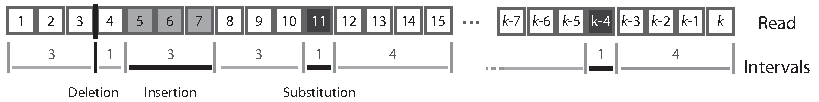
\includegraphics[scale=0.88]{sketch_seeding.pdf}
\caption{\textbf{Structure of reads}. Here we consider sequencing reads
that can have any type of error (insertions, deletions or substitutions).
The reads have size $k$, and the errors are represented as grey squares. A
read is composed of error-free intervals and error-only intervals. Note
that a deletion is an error-only interval of size $0$, so two error-free
intervals can be contiguous (between position $3$ and $4$ in this
example). However error-free intervals have size at least $1$, so two
error-only intervals cannot be contiguous.}
\label{fig:sketchseed}
\end{figure}

Error-free stretches are particularly important because they faithfully
represent the molecule that was sequenced. If they are long, it is
relatively easy to identify the molecule based on the decoded sequence
because the information content is high, but if they are short, it usually
proves more difficult. For instance, modern mapping algorithms are based
on exact searches, using either hash tables or indexes based on the
Burrows-Wheeler transform, so error-free stretches directly influence the
performance of the alrogithm.

In what follows, the feature of interest is the size of the longest
error-free stretch. To facilitate the discussion, we need to introduce
some terms that will be used throughout.

\begin{definition}
\label{def:error-free-interval}
An \textbf{error-free interval} is a nonempty sequence of correct calls
that cannot be extended left or right.
\end{definition}

In other words, an error-free interval contains no error, and it is
flanked by either an error, or by the end of the read. It is important to
highlight that error-free intervals should really be called ``maximal
error-free intervals''. We dropped ``maximal'' for simplicity because we
have no use for non maximal error-free intervals. In the read shown in
figure~\ref{fig:sketchseed}, the leftmost error-free interval has size
$3$, the next has size $1$, the next has size $3$ and the next has size
$4$.

\begin{definition}
\label{def:seed}
An \textbf{exact $d$-seed} is an error-free interval of size at least $d$.
\end{definition}

In what follows, we will refer to a $d$-seed as simply a ``seed''
whenever the value of $d$ is clear from the context or irrelevant.

Our goal here is to estimate the probability that a read contains a seed.
This obviously depends on the size of the read and on the error rate, but
also on the types of errors. Below we develop a general approach to answer
this question building on the tools developed in
section~\ref{sec:anal}.

The strategy is to first exhibit the weighted generating functions of
reads that contain no seed and then use proposition~\ref{th:ass} to
approximate their probability of occurrence.

Observe that a read is a sequence of error-free intervals, interspersed
with errors. This observation motivates us to use transfer matrices to
express the weighted generating function of reads in terms of $F(z)$, the
weighted generating function of error-free intervals. With an expression
where $F(z)$ appears explicitly, we can then replace it by $F_d(z)$, the
weighted generating function of error-free intervals of size smaller than
$d$. This the corresponds to sequences of ``small'' error-free intervals
interspersed with errors, \textit{i.e.} to reads without seed.

To introduce the concepts progressively, we first describe simplified
models where some types of errors are disallowed. We then describe the
more complex models.





%%%%%%%%%%%%%%%%%% Substitutions only %%%%%%%%%%%%%%%%%%%

\subsection{Substitutions only}
\label{sec:substitutions}

One of the simplest and yet useful models is to assume that errors consist
of substitutions only, and that they occur with the same probability $p$
for every nucleotide. This describes reasonably well the error model of
the Illumina platforms (where $p$ is around $0.01$).
Figure~\ref{fig:subonly} shows the transition probabilities between
correct nucleotides and error-free nucleotides.

\begin{figure}[h]
\centering
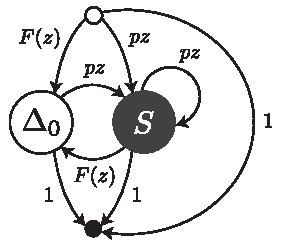
\includegraphics[scale=0.9]{substitutions_only.pdf}
\caption{\textbf{Substitutions only}. 
The substitution rate $p$ is assumed to be constant throughout the read.
Every decoded nucleotide is correct with probability $q = 1-p$.}
\label{fig:subonly}
\end{figure}

With these assumptions, the weighted generating function of mismatches is
$pz$ and that of correct call is $qz$, where $q=1-p$. Since 
error-free intervals are nonempty sequences of correct calls, their
weighted generating function is simply

\begin{equation}
\label{eq:Fsub}
F(z) = qz + (qz)^2 + (qz)^3 + \ldots = \frac{qz}{1-qz}.
\end{equation}

An error-free interval cannot follow another error-free interval,
otherwise one of them could be extended. So an error-free interval must be
followed by a substitution. On the other hand, a substitution can be
followed by either an error-free interval or another substitution. So the
transfer matrix for the states ``match'' and ``substitution'' is

\begin{equation*}
M(z) = \left(
\begin{matrix}
0    & pz \\
F(z) & pz
\end{matrix}
\right).
\end{equation*}

To find the weighted generating function of reads from
proposition~\ref{th:TM2WGF}, we need to find the inverse of $I-M(z)$.
Since $M(z)$ is a $2 \times 2$ matrix, this is straightforward and we
obtain

\begin{equation*}
M_*(z) = (I-M(z))^{-1}=
\frac{1}{\lambda(z)}
\left(
\begin{matrix}
1-pz & pz   \\
F(z) & 1
\end{matrix}
\right)
\end{equation*}

\noindent
where $\lambda(z) = 1-pz(1+F(z))$ is the determinant of $I-M(z)$. Applying
proposition~\ref{th:TM2WGF} with $U(z)$ equal to the row vector $(F(z),
pz)$ and $V$ the column vector equal to $(1,1)$, the weighted generating
function of reads is

\begin{equation}
\label{eq:Ssub}
R(z) = 1 + U(z) \cdot M_*(z) \cdot V = 
\frac{1+F(z)}{1-pz(1+F(z))} = \frac{1}{1-z}.
\end{equation}

Since $1/(1-z) = 1+z+z^2 + \ldots$, this means that the total weight of
reads of size $k$ is equal to $1$ for every finite $k$. This is convenient
because the probability that a read is seedless is the total weight of
seedless reads divided by the total weight of reads, which in this case is
simply equal to the total weight of seedless reads.

To find the weighted generating function of seedless reads, we need to
limit error-free intervals to a maximum size of $d-1$, \textit{i.e.} to
replace $F(z)$ by its truncation $F_d(z) = qz + (qz)^2 + \ldots
+ (qz)^{d-1}$. We obtain

\begin{equation}
\label{eq:Sp}
S(z) = \frac{1+F_d(z)}{1-pz\big( 1+F_d(z) \big)} =
\frac{1+qz + \ldots + (qz)^{d-1}}{1-pz \big(1+qz + \ldots +
(qz)^{d-1} \big)}.
\end{equation}

The task is now to extract the coefficient of $z^k$ in the series
expansion of expression (\ref{eq:Sp}). Instead of the exact solution, we
look for an asymptotic estimate using proposition~\ref{th:ass}. For this,
we need to find the singularities of $S(z)$.

To higlight some general features of the problem, we start with a concrete
case. The left panel of Figure~\ref{fig:plotQ} shows the values of the
denominator of $S(x)$ with $p=0.1$ and $d=17$ for real $x$ around $0$. $S$
has one real root greater than $1$.  The remaining singularities of $S$
are complex and they seem to be evenly spaced on the same circle, as can
be seen on the right panel of Figure~\ref{fig:plotQ}.  This is only a
visual impression.  In fact the singularities are not exactly on the same
circle and their rotation angles are not exactly regular.

\begin{figure}[h]
\centering
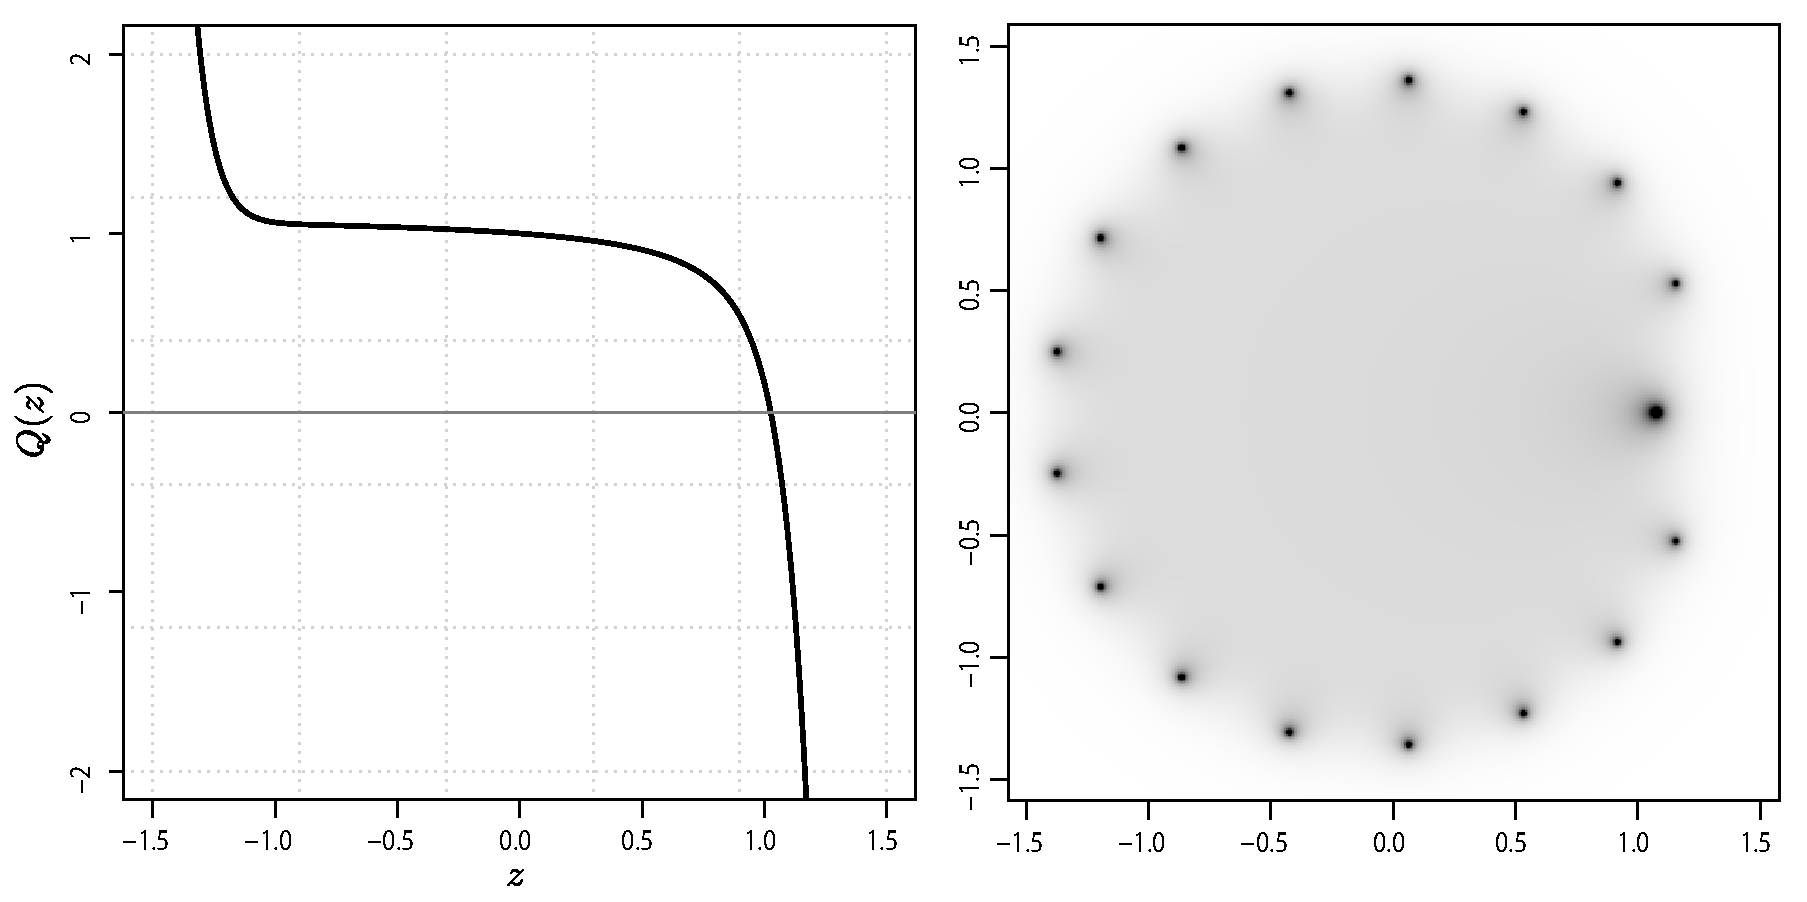
\includegraphics[scale=0.4]{singularityS.pdf}
\caption{\textbf{Singularities of $S$}. $Q(z)$ denotes the
denominator of $S(z)$ from expression (\ref{eq:Sp}) with $p=0.01$ and
$d=17$. \textit{Left}: The value of $Q(z)$ is represented for $z$ real by
the bold line. \textit{Right}: The value of $|1/Q(z)|$ is represented for
$z$ complex by the heat map on the complex plane. Darker pixels correspond
to higher values. Sixteen singularities of $S$ lie close to a circle. The
remaining seventeenth is the one shown on the left panel. It is the
dominant singularity because it is the closest to the origin.}
\label{fig:plotQ}
\end{figure}

It is fortunate that the dominant root of $S$ is a real number because we
can use efficient numerical methods to approximate it (\textit{e.g.}
bisection or the Newton-Raphson method). The following proposition shows
that this is no accident: the dominant singularity of $S$ is always a real
positive number greater than $1$.

\begin{proposition}
\label{th:roots}
$S$ as expressed in (\ref{eq:Sp}) has exactly one positive real
singularity. This is the dominant singularity and it is greater than $1$.
\end{proposition}

\begin{proof}
Write $S(z) = P(z)/Q(z)$ and search the roots of $Q$. First we show that
$Q$ has no real root in the interval $(0,1)$. For a real number $x$ such
that $0\leq x \leq 1$, we have $1+qx+\ldots+(qx)^{d-1} < 1/p$, so $Q(x) >
0$.

Second, we show that $Q$ has exactly one real root great than $1$. Because
$Q'(x) < 0$ for $x \geq 0$ there can ben only one positive root.  Since
$Q(1) = q^d > 0$ and $\lim_{x\rightarrow \infty} Q(x) = -\infty$, $Q$
vanishes for a real number greater than $1$.

Third, we show that this is the root with smallest modulus.  Express the
complex roots of $Q$ as $Re^{i\theta}$. They satisfy the equation

\begin{equation*}
1-pRe^{i\theta}\frac{1-q^dR^de^{id\theta}}{1-qRe^{i\theta}} = 0,
Re^{i\theta} \neq \frac{1}{q}.
\end{equation*}

Multiplying through by $1-qRe^{i\theta}$, we obtain an equation of which
we separate the real and the imaginary parts to obtain

\begin{equation*}
\left\{
\begin{array}{ll}
R \cos (\theta) -1 = pq^dR^{d+1} \cos \left( (d+1) \theta) \right) \\
R \sin (\theta) = pq^dR^{d+1} \sin \left( (d+1) \theta) \right)
\end{array}
\right. Re^{i\theta} \neq \frac{1}{q}.
\end{equation*}

Squaring and summing, we obtain the following equation

\begin{equation*}
R^2 = (pq^dR^{d+1})^2 + 2R \cos(\theta) -1.
\end{equation*}

Since $R > 0$, the solution of this equation is minimal when
$2R\cos(\theta)$ is maximal, \textit{i.e.} when $\theta = 0$. In other
words, the root with smallest modulus is a positive real number. We have
seen above that there exsists exactly one and that it is greater than $1$.
\end{proof}

We now have all the tools to approximate the coefficients of $S(z)$ using
proposition~\ref{th:ass} and thus obtain the approximate probability that
a read contains no seed.

\begin{proposition}
\label{th:p}
The probability that a read of of size $k$ is seedless is
asymptotically equivalent to

\begin{equation*}
\frac{C}{z_1^{k+2}},
\end{equation*}

\noindent
where $z_1$ is the only real positive root of the denominator of $S(z)$,
\textit{i.e.} the root of $1-pz(1+qz+\ldots+(qz)^{d-1})$, and where

\begin{equation}
\label{eq:Cp}
C =\frac{(1-qz_1)^2}{p^2\big( 1-(d+1-dqz_1)(qz_1)^d \big)}.
\end{equation}
\end{proposition}

\begin{proof}
Apply propositions~\ref{th:ass} and \ref{th:roots}, together with the fact
that for any singularity $z$ we have $1+qz+\ldots+(qz)^{d-1} = 1/pz$.
\end{proof}

We now illustrate proposition~\ref{th:p} with a concrete example
explaining how the calculations are done in practice.

\begin{example}
\label{ex:num1}
Let us approximate the probability that a read of size $k=100$ is seedless
for $d=17$ and for a substitution rate $p=0.1$. To find the dominant
singularity of $S$, we need to solve
$1-0.1z\times(1+0.9z+\ldots+(0.9z)^{16}) = 0$.  We rewrite the equation as
$1 - 0.1z\times(1-(0.9 z)^{17})/(1-0.9z) = 0$ and use bisection to solve
it numerically, yielding $z_1 \approx 1.0268856$. Substituting this value
in (\ref{eq:Cp}) yields $C \approx 1.433681$, so the probability that a
read contains no seed is approximately $1.433681 / 1.0268856^{102} \approx
0.095763$. For comparison, a 99\% confidence interval obtained by
performing 10 billion random simulations is $0.09575-0.09577$.
% The magic number is 957598614 out of 10 billion.
\end{example}

\begin{figure}[h]
\centering
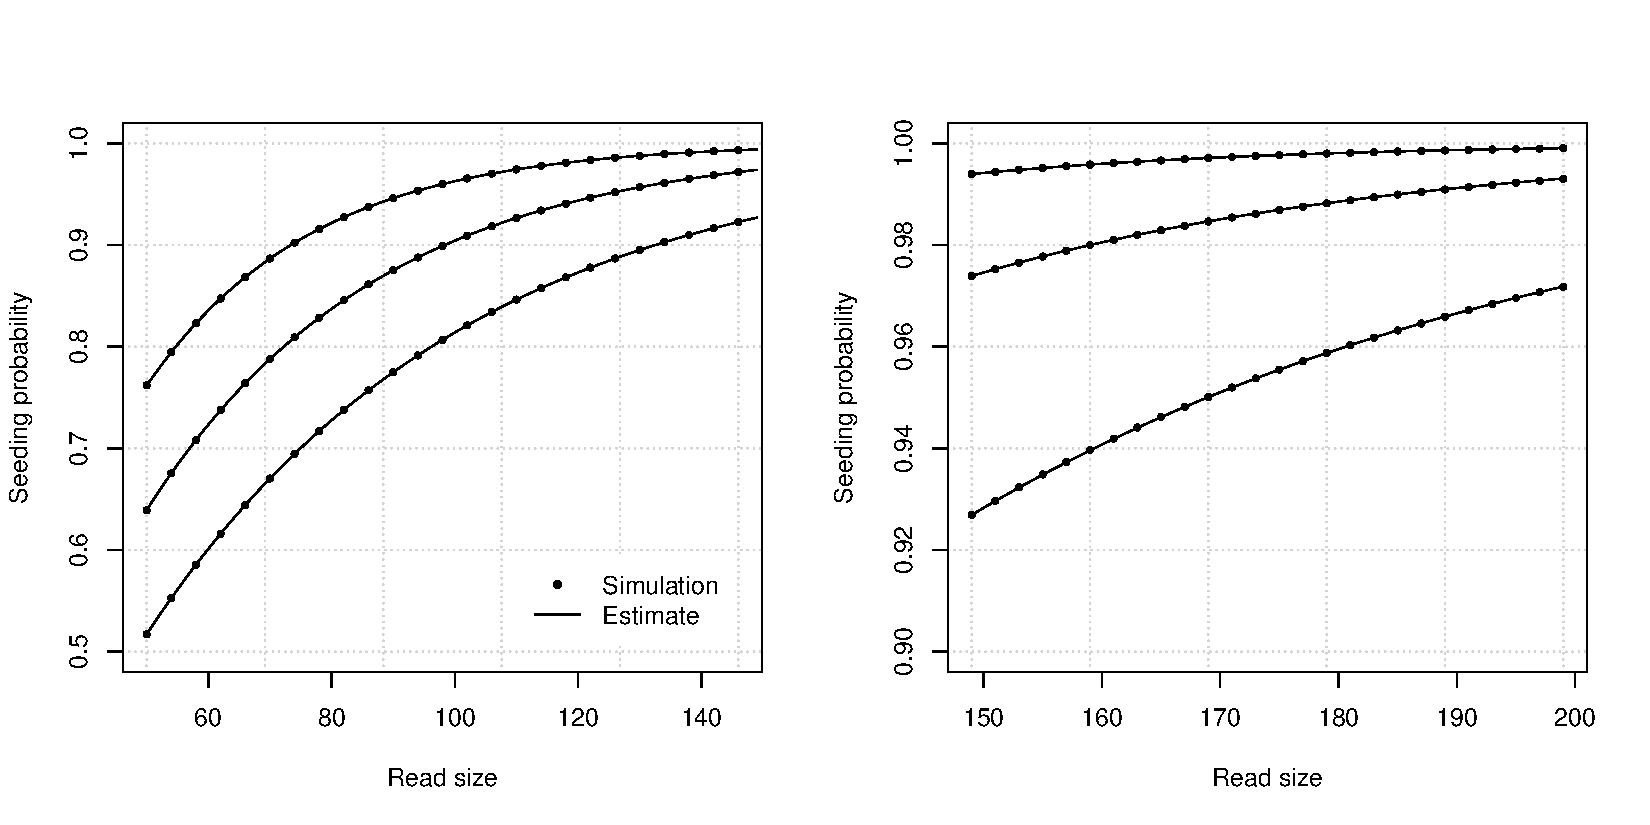
\includegraphics[scale=0.445]{simulp.pdf}
\caption{\textbf{Example estimates for substitutions only}. The analytic
combinatorics estimates of proposition~\ref{th:p} are benchmarked against
random simulations. Shown on both panels are the probablities that a read
of given size contains a seed, either estimated by 10,000,000 random
simulations (dots), or by the method described above (lines). The curves
are drawn for $d=17$ and $p=0.08$, $p=0.10$ or $p=0.12$ (from top to
bottom). The difference never exceeds 0.0003 on the examples shown here,
which is the expected variation for this number of random trials.}
\label{fig:simulp}
\end{figure}

Overall, the analytic combinatorics estimates are close to the exact
values. Figure~\ref{fig:simulp} also shows that relatively small changes
in the prboability of error have a large influence on the probability of
that the read contains a seed in the depicted range of read sizes.



%%%%%%%%%%%%%%%%% Subsitutions and deletions %%%%%%%%%%%%%%%%%%

\subsection{Substitutions and deletions}
\label{sec:deletions}

The uniform substitution model does not describe all sequencing
technologies. For instance, long read technologies often have bursts of
insertions and deletions, with typical frequencies that differ from
substitutions. In order to model more complex behaviors, we need to
distinguish the different types of errors.

To not jump too fast into the difficulties, we will first focus on the
semi-realistic case where errors can be deletions or susbtitutions, but
not insertions. As in the case of uniform substitutions, we assume that
every nucletoide call is false with a probability $p$ and true with a
probability $1-p=q$. Here, we also assume the ``space''  between
consecutive nucleotides can contain a deletion with probability $\delta$.

A deletion may be adjacent to a substitution, or lie in between two
correct nucleotides. In the first case, the deletion does not interrupt
any error-free intervals so it does not change the probability that the
read contains a seed. For this reason, we ignore deletions next to
substitutions. More precisely, we assume that they can occur, but whether
they do has no importance for the problem.

Figure~\ref{fig:deletions}
shows the transition probabilities between errors and correct calls. As
mentioned above, a substitution can be followed or preceded by a deletion
(each with probability $\delta$), but this information is regarded for
simplicity. Only the self transition of the state ``Match'' needs to
explicitly distinguish whether it contains a deletion.

\begin{figure}[h]
\centering
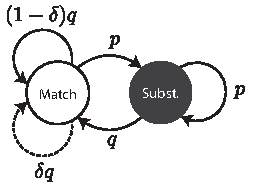
\includegraphics[scale=0.9]{deletions.pdf}
\caption{\textbf{Substitutions and deletions}. 
Substitution and deletion rates $\delta$ and $p$ are assumed to be
constant throughout the read. Deletions do not have a state of their own
because they have size $0$ and never ``appear'' in the structure of the
read. Deletions before or after a substitution are ignored because they
have no effect on the error-free intervals. For instance, the transition
from ``Match'' to ``Substitution'' is $\delta p + (1-\delta)p = p$. The
same holds for the other transitions to and from ``Substitution''.}
\label{fig:deletions}
\end{figure}

The weighted generating function of error-free intervals of size $1$ is
simply $qz$. They are either at the beginning of the read or after a
substitution and in both cases deletions are irrelevant. For an error-free
interval of size $k$, we must ensure that there is no deletion in the
$k-1$ ``spaces'' between the nucleotide calls, so the weighted generating
function is $(1-\delta)^{k-1}(qz)^k$. Summing for all the possible sizes,
we obtain the weighted generating function of error-free intervals as

\begin{equation}
\label{eq:Fdel}
F(z) = qz + (1-\delta)(qz)^2 + (1-\delta)^2(qz)^3 \ldots =
\frac{qz}{1-(1-\delta)qz}.
\end{equation}

The only difference with the transwer matrix of
section~\ref{sec:substitutions} is that an error-free interval can follow
another error-free interval, provided there is a deletion between them.
Since the weight of this deletion is $\delta$, the transfer matrix is

\begin{equation*}
M(z) = \left(
\begin{matrix}
\delta F(z) & pz \\
F(z)        & pz
\end{matrix}
\right).
\end{equation*}

To apply proposition~\ref{th:TM2WGF} we need to invert $I-M(z)$, which is
straightforward for a $2 \times 2$ matrix. We obtain

\begin{equation*}
M_*(z) = (I-M(z))^{-1}=
\frac{1}{\lambda(z)}
\left(
\begin{matrix}
1-pz  & pz              \\
F(z) & 1 -\delta F(z)
\end{matrix}
\right),
\end{equation*}

\noindent
where $\lambda(z) = 1-pz-(pz(1-\delta)+\delta)F(z)$ is the determinant of
$I-M(z)$.

As in section~\ref{sec:substitutions}, the row vector $U(z)$ of starting
states is $(F(z), pz)$, and the column vector of end states is $(1,1)$, so
we obtain the weighted generating function of reads as

\begin{equation}
\label{eq:Sdel}
\begin{split}
R(z) &= 1 + U(z) \cdot M_*(z) \cdot V \\
&= \frac{1+(1-\delta)F(z)} {1-pz - \big(pz(1-\delta) + \delta\big)F(z)}
= \frac{1}{1-z}.
\end{split}
\end{equation}

The terms of equation (\ref{eq:Sdel}) cancel out when $F$ is defined as in
(\ref{eq:Fdel}). The result is $1/(1-z) = 1+z +z^2 + \ldots$, which means
that the total weight of reads of size $k$ is equal to $1$ for every $k
\geq 0$.

To find the weighted generating function of seedless reads, we need to
limit error-free intervals to a maximum size of $d-1$, \textit{i.e.} to
replace $F(z)$ by its truncation $F_d(z) = qz + (1-\delta)(qz)^2 + \ldots
+ (1-\delta)^{d-2}(qz)^{d-1}$. With this definition, the weighted
generating function of seedless reads is

\begin{equation}
\label{eq:Sdel}
S(z) = \frac{1+(1-\delta)F_d(z)}
  {1-pz - \big(pz(1-\delta) + \delta\big)F_d(z)}.
\end{equation}

Applying proposition~\ref{th:ass} to this expression, we obtain the
following proposition.

\begin{proposition}
\label{th:pd}
The probability that a read of size $k$ is seedless is asymptotically
equivalent to

\begin{equation*}
\frac{C}{z_1^k},
\end{equation*}

\noindent
where $z_1$ is the only real positive root of the denominator of $S(z)$,
\textit{i.e.} the root of $1-pz - \big(pz(1-\delta) +
\delta\big)\big(qz+(1-\delta)(qz)^2 + \ldots +
(1-\delta)^{d-2}(qz)^{d-1}\big)$, and

\begin{equation}
\label{eq:Cpd}
\begin{split}
C &=
\frac{ \big(1-(1-\delta)(1-p)z_1\big)^2 }
{ \big((p+q\delta)z_1  -\gamma^*(1-\delta)^{d-1}(qz_1)^d \big)
\big(\delta+(1-\delta)pz_1\big) }, \\
\gamma^* &= d\delta -(1-\delta)\big((d-1)\delta-p((d-1)\delta+d+1)\big)z_1
- d(1-\delta)^2pqz_1^2.
\end{split}
\end{equation}
\end{proposition}

\begin{remark}
Notice that the power of $z_1$ differs between propositions~\ref{th:p} and
\ref{th:pd}. The reason is that the factors $z$ or $1/z$ have been moved
out of the constant $C$ in expressions (\ref{eq:Cp}) and (\ref{eq:Cpd}).
\end{remark}

\begin{example}
\label{ex:num2}
Let us approximate the probablity that a read of size $k = 100$ is
seedless for $d=17$, $p = 0.05$ and $\delta = 0.15$. In order to find the
dominant singularity of $S$ expressed as (\ref{eq:Sdel}), we need to solve
the equation $1-0.05z - \big(0.0425z + 0.15\big) \big(0.95z+0.85(0.95z)^2
+ \ldots + 0.85^{15}(0.95z)^{16}\big) = 0$. We write it as $1-0.05z -
\big(0.0425z + 0.15) (0.95z-0.85^{16}(0.95z)^{17}) / (1-0.8075z) = 0$ and
use bisection to solve it, yielding $z_1 \approx 1.006705$. Now
substituting the obtained value in (\ref{eq:Cpd}) gives $C \approx
1.088876$, so the probability that a read contains no seed is
approximately $1.088876 / 1.006705^{100} \approx 0.558141$. For
comparison, a 99\% confidence interval obtained by performing 10 billion
random simulations is $0.55813-0.55816$.
% The magic number is 5581417733 out of 10 billion.
\end{example}

\begin{figure}[h]
\centering
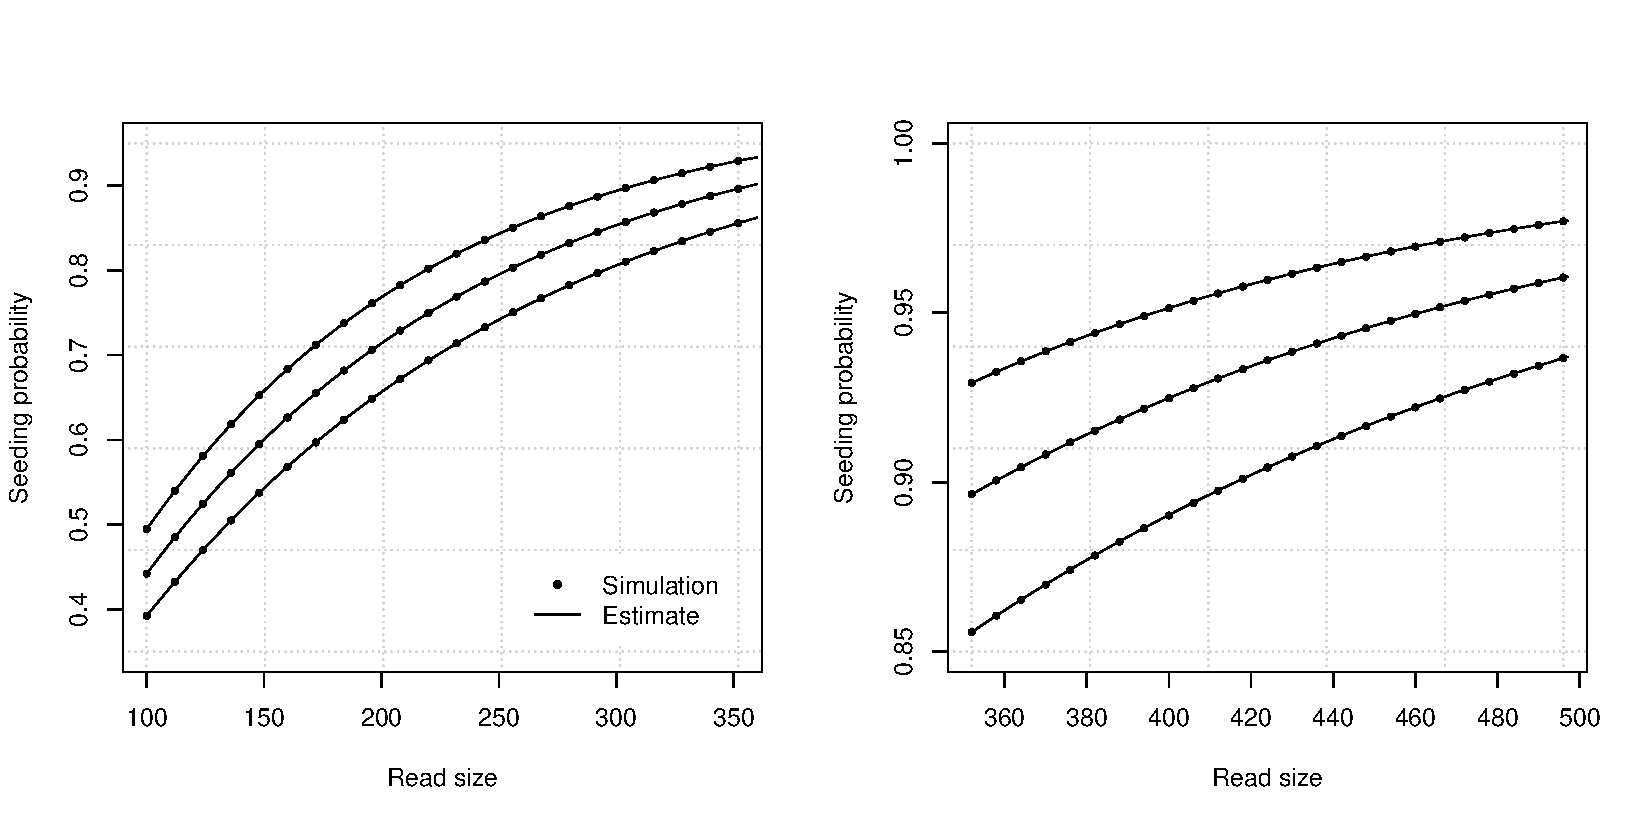
\includegraphics[scale=0.445]{simulpdel.pdf}
\caption{\textbf{Example estimates for substitutions and deletions}. The
analytic combinatorics estimates of proposition~\ref{th:pd} are
benchmarked against random simulations. Shown on both panels are the
probablities that a read of given size contains a seed, either estimated
by 10,000,000 random simulations (dots), or by the method described above
(lines). The curves are drawn for $d=17$, $p=0.05$ and $\delta=0.14$,
$\delta=0.15$ or $\delta=0.16$ (from top to bottom). The difference never
exceeds 0.0003 on the examples shown here, which is the expected variation
for this number of random trials.}
\label{fig:simulpdel}
\end{figure}




%%%%%%%%%%% Subsitutions, deletions and insertions %%%%%%%%%%%%

\subsection{Substitutions, deletions and insertions}
\label{subsec:sdi}

Introducing insertions brings two additional difficulties. The first is
that substitution is indistinguishable from an insertion followed by a
deletion (or a deletion followed by an insertion). By convention, we will
count all these cases as substitutions. This entails that a deletion can
never be found next to an insertion. The second difficulty is that
insertions usually come in bursts. This is also the case of deletions, but
we could neglect it because this does not affect the size of the interval
(all deletions have size $0$). 

We still denote the probability of substitution as $p$ and the probability
of deletion $\delta$. To model insertion bursts, we need to assign a
probability $r$ to the first insertion, and a probability $\tilde{r} > r$
to all subsequent insertions of the burst. We will still denote the
probability of a correct call as $q$, but here $q = 1-p-r$.  An insertion
burst stops with probability $1-\tilde{r}$ at each position, sandt is
followed by either a match or a substitution with probability $1-p/(1-r) =
q/(1-r)$ and $p/(1-r)$, respectively. Figure~\ref{fig:insertions} shows
the transition probabilities between matches, substitutions and
insertions.

\begin{figure}[h]
\centering
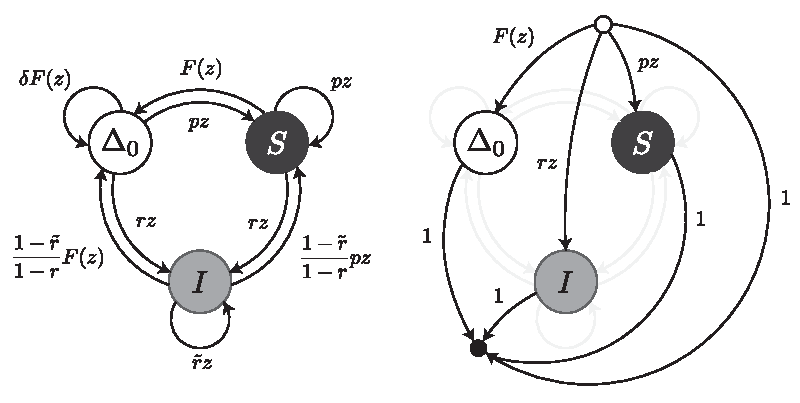
\includegraphics[scale=0.9]{insertions.pdf}
\caption{\textbf{Substitutions, deletions and insertions}. Rates of
substitution ($p$), deletion ($\delta$) and insertion ($r$) are assumed to
be contant throughout the read. The prolongation rate of insertions
($\tilde{r}$) is also assumed to be constant. Here $q = 1-p-r$ and the
transitions from ``Inertion'' to ``Match'' and ``Substitution'' are
normalized to maintain a constant rate of substitution.}
\label{fig:insertions}
\end{figure}

As in section\ref{sec:deletions}, we must ensure that there is no deletion
between any two positions of an error-free interval. The weighted
generating function thus comes as

\begin{equation*}
F(z) = qz + (1-\delta)(qz)^2 + (1-\delta)^2(qz)^3 \ldots =
\frac{qz}{1-(1-\delta)qz}.
\end{equation*}

This expression is the same as in the case of section\ref{sec:deletions},
but here $q = 1-p-r$ instead of $1-p$. Based on the error model and the
conventions, the transfer matrix for the states ``match'',
``substitution'' and ``insertion'' is

\begin{equation*}
M(z) = \left(
\begin{matrix}
\delta F(z) & pz      & rz  \\
F(z)        & pz      & rz  \\
\frac{1-\tilde{r}}{1-r}F(z)   & \frac{1-\tilde{r}}{1-r}pz & \tilde{r}z
\end{matrix}
\right).
\end{equation*}

The expression of $M_*(z) = (I-M(z))^{-1}$ is omitted because it is
cumbersome and all we need is the value if $1+U(z)\cdot M_*(z)\cdot V$.
We still give the determinant of $I-M(z)$ in full because this will be the
denomiator of the final expression. Up to a factor $1-r$, it is equal to
$1-a(z)-b(z)F(z)$, where

\begin{gather}
\label{eq:a+b}
a(z) = r-\big((p+\tilde{r})r-\tilde{r}-p\big)z
- p(\tilde{r}-r)z^2\text{, and} \\
b(z) = \delta(1-r) - \big((\tilde{r}\delta-(1-\delta)p)(1-r)
-(1-\tilde{r})r\big)z -(1-\delta)p(\tilde{r}-r)z^2.
\notag
\end{gather}

Applying proposition~\ref{th:TM2WGF} the weighted generating function of
reads appears as

\begin{equation}
\label{eq:Rindel}
\begin{split}
R(z) &= 1 + U(z) \cdot M_*(z) \cdot V \\
&= \frac{(1-r)\big( 1-(\tilde{r}-r)z \big)
\left(1+(1-\delta)F(z) \right)}{1-a(z)-b(z)F(z)}
= \frac{1}{1-z}.
\end{split}
\end{equation}

Again, the terms cancel out and we obtain the simple expression
$1/(1-z)$ where all the coefficients are equal to $1$. To find the
weighted generating function of seedless reads, we replace $F(z)$ in
expression (\ref{eq:Rindel}) by its truncated version

\begin{equation*}
\begin{split}
F_d(z) &= qz + (1-\delta)(qz)^2 + (1-\delta)^2(qz)^3 \ldots +
(1-\delta)^{d-2}(qz)^{d-1} \\
&= \frac{qz-(1-\delta)^{d-1}(qz)^d}{1-(1-\delta)qz}.
\end{split}
\end{equation*}

We obtain the following expression

\begin{equation}
\label{eq:Sindel}
S(z) = \frac{(1-r)\big( 1-(\tilde{r}-r)z \big) \left(1+(1-\delta)F_d(z)
\right)}{1-a(z)-b(z)F_d(z)},
\end{equation}

\noindent
where the terms $a(z)$ and $b(z)$ are defined in (\ref{eq:a+b}).

\begin{proposition}
\label{th:pins}
The probability that a read of size $k$ is seedless is asymptotically
equivalent to

\begin{equation*}
\frac{C}{z_1^{k+1}},
\end{equation*}

\noindent
where $z_1$ is the only real positive root of the polynomial
$1-a(z)-b(z)F_d(z) = 1-a(z)-b(z)\big(qz+(1-\delta)(qz)^2 + \ldots +
(1-\delta)^{d-2}(qz)^{d-1}\big)$, and $C = \alpha / \beta$, with

\begin{equation*}
\alpha = (1-r)(1-(\tilde{r}-r)z_1)
   \frac{1-\big((1-\delta)(qz)\big)^d}{1-(1-\delta)qz}
\end{equation*}

\noindent
and
\begin{equation*}
\begin{split}
\beta = a'(z_1) &- \left( b'(z_1) +
\frac{(1-\delta)q}{1-(1-\delta)qz}\right)
\frac{qz-(1-\delta)^{d-1}(qz)^d}{1-(1-\delta)qz} \\
&+b(z_1) \frac{q-d(1-\delta)^{d-1}q^dz^{d-1}}{1-(1-\delta)qz}.
\end{split}
\end{equation*}
\end{proposition}

Note that the constant $C$ above has an explicit expression for a given
value of $z_1$, but it is relatively cumbersome, so it is more useful to
show how to compute it. We now show how to apply propostion~\ref{th:pins} in a
practical case.

\begin{example}
\label{ex:num3}
Let us approximate the probability that a read of size $k=100$ is seedless
for $d=17$ for $p=0.05$, $\delta=0.15$, $r=0.05$ and $\tilde{r}=0.45$.
With these values, $a(z) = 0.05 +0.475z -0.02z^2$ and $b(z) = 0.1425 +
0.00375z-0.017z^2$. We need to solve $0.95-0.475z+0.02z^2 - (0.1425
+0.00375z-0.017z^2)(0.9z+0.85(0.9z)^2+\ldots+0.85^{15}(0.9z)^{16}) = 0$.
We rewrite the equation as $0.95-0.475z+0.02z^2 - (0.1425
+0.00375z-0.017z^2)(0.9z-0.85^{15}(0.9z)^{16})/(1-0.765z) = 0$ and use
bisection to solve it numerically, yielding $z_1 \approx 1.00295617$.
Using proposition~\ref{th:pins}, we obtain $C \approx 1.042504$, so the
probability that a read contains no seed is approximately $1.042504 /
1.00295617^{101} \approx 0.773749$. For comparison, a 99\% confidence
interval obtained by performing 10 billion random simulations is
$0.77373-0.77376$.
% The magic number is 7737489777 out of 10 billion.
\end{example}

\begin{figure}[h]
\centering
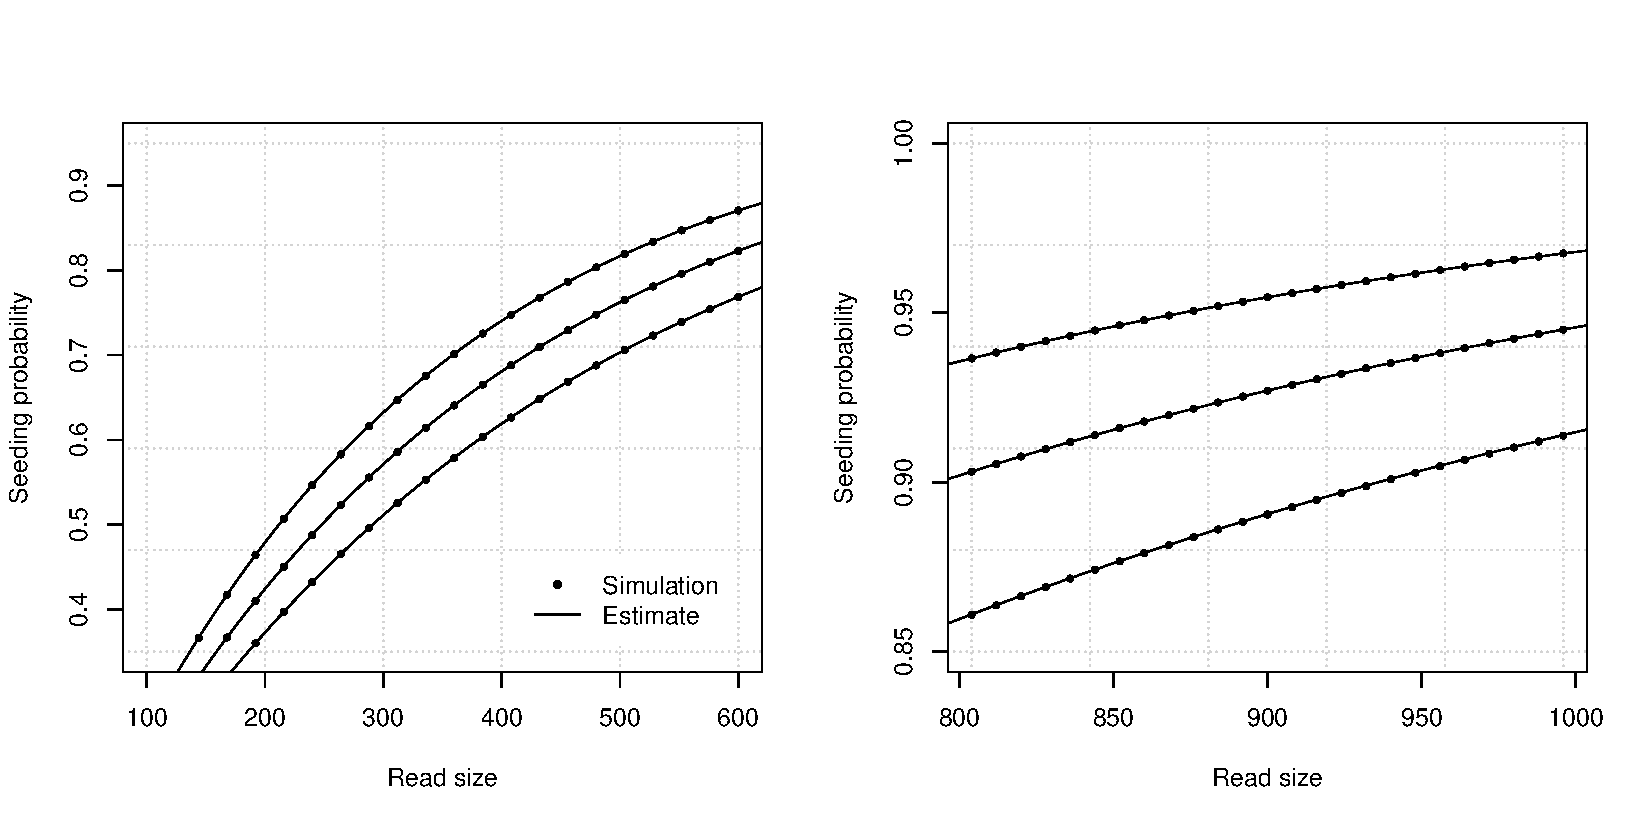
\includegraphics[scale=0.445]{simulpins.pdf}
\label{fig:simulpins}
\caption{\textbf{Example estimates for substitutions, deletions and
insertions}. The analytic combinatorics estimates of
proposition~\ref{th:pins} are benchmarked against random simulations.
Shown on both panels are the probablities that a read of given size
contains a seed, either estimated by 10,000,000 random simulations (dots),
or by the method described above (lines). The curves are drawn for $d=17$,
$p=0.05$, $\delta=0.15$, $\tilde{r} = 0.45$ and $r=0.04$, $r=0.05$ or
$r=0.06$ (from top to bottom). The difference never exceeds 0.0002 on the
examples shown here, which is the expected variation for this number of
random trials.}
\end{figure}


\begin{remark}
Note that when $r = \tilde{r} = 0$, $a(z) = pz$ and $b(z) = pz(1-\delta) +
\delta$, so expression (\ref{eq:Sindel}) becomes

\begin{equation*}
S(z) = \frac{1 + (1-\delta)F_d(z)}{1-pz-(pz(1-\delta)+\delta))F_d(z)}.
\end{equation*}

This is expression (\ref{eq:Sdel}), \textit{i.e.} the model described in
section~\ref{sec:deletions}. When we also have $\delta = 0$, this
expression further simplifies to

\begin{equation*}
S(z) = \frac{1 + F_d(z)}{1-pz(1 + F_d(z))}.
\end{equation*}

This is expression (\ref{eq:Sp}), \textit{i.e.} the model described in
section~\ref{sec:substitutions}. In other words, the error models
described previously are special cases of this one.
\end{remark}



%%%%%%%%%%%%%%%%%%%% Empirical error models %%%%%%%%%%%%%%%%%%

\subsection{Empirical error models}
\label{subsec:empirical}

In the theory developed here, the only variable of interest is the
probability distribution of the error intervals. Indeed, the only reason
we introduced different kinds of errors is because they have different
probabilities and different sizes, but the nature of the error is
irrelevant.

In addition to error-free intervlas, we introduce error-only intervals,
which will encapsulate the available information about the size of error
patches. As we will see below, we need to keep error-free intervals and
deletions separate, so error-only intervals are always considered to be
nonempty.

\begin{definition}
\label{def:error-interval}
An \textbf{error-only interval} is a nonempty sequence of errors that
cannot be extended left or right.
\end{definition}

If we have empirical probabilities $p_0, p_1, \ldots, p_n$ such that $p_k$
is the probability that the error pach has size $k$, we can directly write
the weighted generating function of nonempty error intervals as $E(z) =
p_1z + p_2z^2 + \ldots + p_nz^n$. If the terms are estimated by averaging
observations, this function is a polynomial and $n$ is the size of largest
observed error patch.

The weighted generating function of deletions is simply $p_0$. We will set
$\delta = p_0$ for consistency with the previous sections. We need to keep
deletions separate from error-only intervals because a read cannot start
or end with a deletion (there is no way to detect them before the read
starts or after it finishes). For this reason, we must keep one extra
state of the transfer matrix for deletions. But we must remember that an
uninterrupted error patch was either a deletion or an error-only interval,
so deletions and error-free intervals cannot lie next to each other.

An error-free interval can be followed by an error-only interval or by a
deletion, but it cannot be followed by another error-free interval. An
error-only interval can only be followed by an error-free interval.
Similarly, a deletion can only be followed by an error-free inerval. The
transfer matrix of the objects ``error-free interval'', ``error-only
interval'' and ``deletion'' is

\begin{equation*}
M(z) = \left(
\begin{matrix}
0    & E(z) & \delta  \\
F(z) & 0    & 0       \\
F(z) & 0    & 0
\end{matrix}
\right).
\end{equation*}

Since the sequence may neither start nor end with a deletion, the row
vector of start objects $U(z)$ is equal to $(F(z), E(z), 0)$ and the
column vector $V$ of end objects is equal to $(1,1,0)$. The weighted
generating function of reads can be expressed in general terms as

\begin{equation}
\label{eq:Remp_gen}
R(z) = 1 + U(z) \cdot (I-M(z))^{-1} \cdot V =
\frac{\big(1+(1-\delta)F(z)\big)\big(1+E(z)\big)}
   {1-F(z)\big(\delta+E(z)\big)}.
\end{equation}

As previously, the weighted generating function of error-free intervals is
$F(z) = qz + (1-\delta)(qz)^2 + (1-\delta)^2(qz)^3 + \ldots =
qz/(1-(1-\delta)qz)$. Substituting this value in the equation above, we
obtain

\begin{equation}
\label{eq:Remp}
R(z) = \frac{1+E(z)}{1-qz\big(1+E(z)\big)}.
\end{equation}

Epxression (\ref{eq:Remp}) is not equal to $1/(1-z)$ because $E(z)$ is in
general not equal to $pz/(1-pz)$. This means that the total weight of
reads of size $k$ is not equal to $1$, so we will need to take this
into account in our approximations. As usual, we will use
proposition~\ref{th:ass}, implying that we have to find the root with
smallest modulus of the polynomial $1-qz\big(1+E(z)\big)$.

To find the weighted generating function of seedless reads, we need to
replace $F(z)$ by its truncation $F_d(z) = qz + (1-\delta)(qz)^2 + \ldots
+ (1-\delta)^{d-2}(qz)^{d-1}$ in expression (\ref{eq:Remp_gen}). The terms
only partially cancel each other and we obtain

\begin{equation}
\label{eq:Semp}
S(z) = \frac{\big(1+E(z)\big)\big( 1-(1-\delta)^d(qz)^d \big)}
{1-(1-\delta)qz-qz\big(1-(1-\delta)^{d-1}(qz)^{d-1}\big)
\big(\delta+E(z)\big) }.
\end{equation}

To estimate the total weight of seedless reads, we need to find the root
with smallest modulus of $1-qz\big(1+E(z)\big) +
(1-\delta)^{d-1}(qz)^{d-1}\big(\delta+E(z)\big)$. The solution depends on
the particular expression of $E(z)$. Even though the process can be
automated using proposition~\ref{th:ass}, every case is different and
we cannot give an explicit formula here.

\begin{example}
Assume that a series of empirical measurements suggest that $q = 0.9$,
$\delta = 0.1$ and that error patches have size $1$, $2$ or $3$ have
probabilities $0.5$, $0.33$ and $0.17$. This implies that $E(z) = 0.5z +
0.33z^2+0.17z^3$.

If we choose seeds of size $d=17$, the weighted generating function of
reads show in (\ref{eq:Remp}) becomes

\begin{equation*}
R(z) = \frac{1+0.5z +0.33z^2+0.17z^3}
{1-0.9z\big(1+0.5z +0.33z^2+0.17z^3\big)}.
\end{equation*}

The smallest root of the denominator is approximately equal to $0.1946949$
and applying proposition~\ref{th:ass}, the multiplicative constant is
approximately equal to $1.905695$, so the total weight of reads of size
$k$ is approximately equal to $1.905695/0.1946949^{k+1}$.

Similary, the weighted generating function of seedless reads shown in
(\ref{eq:Semp}) becomes

\begin{equation*}
S(z) = \frac{\big(1+0.5z +0.33z^2+0.17z^3\big)\big( 1-(0.81z)^{17} \big)}
{1-0.81z-0.9z(1-(0.81z)^{16})(0.1+0.5z +0.33z^2+0.17z^3)}.
\end{equation*}

The smallest root of the denominator is approximately $0.0122100$ and the
ultiplicative constant is approximately equal to $0.0135667$. So the total
weight of seedless reads of size $k$ is approximately equal to $0.0135667
/ 0.0122100^{k+1}$.

Combining these two results, we obtain the probability that a read of size
$k$ has no seed as the ratio of the total weights computed above. This is
approximately equal to $0.007119 / 0.06271356^{k+1}$.
\end{example}








%%%%%%%%%%%%%%%%%% sampling seedless reads %%%%%%%%%%%%%%%%%%%%%

\section{Sampling seedless reads}

It is trivial to use the error models presented above to sample reads.
This approach is suboptimal if we are only interested in seedless
reads, because they may be sampled at a very low rate. Sampling
seedless reads at maximum rate, \textit{i.e.} without rejection is
desirable when they occur at low frequency under the given error model.
The question is how to sample the reads with a frequency that is equal to
their expected occurrence among seedless reads.

Here analytic combinatorics offers a simple way to achieve this via the
symbolic method. The combinatorial construction associated with an
error model gives us a handle for a sampling algorithm. At each iteration
of the process, we simulate the length of an error-free interval, which is
a number between $0$ and $d-1$, followed by an error. The probabilities
of these $d$ possible outcomes are computed thanks to asymptotic formulas
given by proposition§~\ref{th:ass}.




\subsection{Substitutions only}
\label{sec:smplsub}

We start from the weighted generating function of seedless reads, namely

\begin{equation}
\tag{\ref{eq:Sp}}
S(z) = \frac{1+F_d(z)}{1-pz\big( 1+F_d(z) \big)}.
\end{equation}

Notice that according to proposition~\ref{th:sequences}, this expression
is also equal to

\begin{equation}
\label{eq:altSp}
\left( \sum_{n=0}^\infty \big( (1+F_d(z))pz \big)^n \right)
  (1+F_d(z)).
\end{equation}

Expression (\ref{eq:altSp}) indicates that a read can be viewed as a
sequence of objects with weighted generating function $(1+F_d(z))pz$,
followed by a single object with weighted generating function $1+F_d(z)$.
Note that $1+F_d(z)$ is the weighted generating function of possibly empty
error-free intervals of size less than $d$, because it is the sum of the
weighted generating functions of the empty object and of error-free
intervals of size less than $d$.

Recalling that $pz$ is the weighted generating function of substitutions,
the term $(1+F_d(z))pz$ now appears as the weighted generating function of
a possibly empty error-free interval of size less than $d$, followed by a
substitution. We introduce this type of combinatorial sequence in the
definition below.

\begin{definition}
A \textbf{substitution interval} is a possibly empty error-free
interval, followed by a substitution.
\end{definition}

\begin{figure}[h]
\centering
\includegraphics[scale=0.89]{sketch_substitution_intervals.pdf}
\caption{\textbf{Decomposition of a read in substitution intervals}. When
errors consist of substitutions only, we can segment reads in substitution
intervals. This decomposition is unique and every substitution belongs to
a unique interval (the last interval may not contain a substitution). In
this example, a read of size $23$ with $4$ substitutions (black squares)
is segmented in $5$ substitution intervals.}
\label{fig:sketchsubint}
\end{figure}

The point of this definition is that by expression (\ref{eq:altSp}), a
read can be decomposed as a sequence of substitution intervals followed by
a possibly empty error-free interval (Figure~\ref{fig:sketchsubint}).

This observation is the key of a method to sample seedless reads. Assume
that the read size $k$, the minimum seed length $d$ and the substitution
rate $p$ are given. We want to generate a read according to its
probability of occurrence among seedless reads.

If the read starts with a substitution interval of size $m$ ($1 \leq m
\leq d$), then it consists of an error-free interval of size $m-1$,
followed by a substitution, followed by a seedless read of size $k-m$.
The probability of such a read is $q^{m-1} \times p \times C/z_1^{k-m+1}$.
Since the occurrence of seedless reads of size $k$ is $C/z_1^{k+1}$, the
probability that a seedless read starts with a substitution interval of
size $m$ is $pz_1(qz_1)^{m-1}$.

Notice that $pz_1 + pz_1qz_1 + \ldots + pz_1(qz_1)^{d-1} = 1$ because by
definition, $z_1$ is a root of the polynomial $1-pz(1+F_d(z)) =
1-pz(1+qz+\ldots+pz_1(qz)^{d-1})$. This shows that the terms
$pz_1(qz_1)^{m-1}$ can be interpreted as probabilities, giving a
straightforward way to sample the first substitution interval. This is a
geometric distribition with parameter $qz_1$, conditioned on the values
$0, 1, \ldots, d-1$.

The process can be repeated to produce the next substitution intervals.
When the generated read has size $k$ or greater, the process is stopped,
and the nucleotides beyond $k$ are removed. The analytic combinatorics
approaches directly yields a simple and efficient scheme to sample
seedless reads. Once again, it is unclear how one may obtain the same
result with a different approach.





\subsection{Substitutions and deletions}

We can use the same principle to sample seedless reads under the error
model descrbibed in section~\ref{sec:deletions}.

\begin{equation}
\tag{\ref{eq:Sdel}}
S(z) = \frac{1+F_d(z)(1-\delta)}{1-pz-\big(pz(1-\delta)
  + \delta\big) F_d(z)}.
\end{equation}

Using proposition~\ref{th:sequences}, can express (\ref{eq:Sdel}) as

\begin{equation*}
  \left( \sum_{n=0}^\infty \left( \frac{F_d(z)
  \big( \delta + (1-\delta)pz \big) }{1-pz}
  \right)^n \right) \frac{1+(1-\delta)F_d(z)}{1-pz}.
\end{equation*}

This shows that under the error model of uniform substitutions and
deletions, reads can be interpreted as sequences of combinatorial objects
with weighted generating function $F_d(z)\big( \delta + (1-\delta)pz \big)
/ (1-pz)$, followed by a combinatorial object with weighted generating
function $(1+F_d(z)(1-\delta))/(1-pz)$.

The first weighted generating function consists of three components. The
term $1/(1-pz)$ is the weighted generating function of sequences of
substitutions (possibly interspersed with deletions). The term $F_d(z)$ is
the weighted generating function of error-free intervals of size less than
$d$. Finally, the term $\delta  + (1-\delta)pz$ is the weighted generating
function of a deletion, or a substitution not preceded by a deletion. We
refer to these components as ``head'', ``body'' and ``tail'',
respectively, which together make a ``deletion interval''
(Figure~\ref{fig:sketchdelint}).

\begin{definition}
A \textbf{deletion interval} is a sequence of deletions (called the head),
followed by an error-free interval (called the body), followed by either a
deletion or a substitution (called the tail).
\end{definition}

\begin{figure}[h]
\centering
\includegraphics[scale=0.89]{sketch_deletion_intervals.pdf}
\caption{\textbf{Decomposition of a read in deletion intervals}. When
errors consist of either substitutions or deletions, we can segment reads
in deletions intervals. \textit{Top:} deletions intervals consist of a
head, a body and a tail. The head is a sequence of substitutions, possibly
interspersed (but not starting) by deletions. THe body is an error-free
interval. The tial is either a deletion, or a substitution (not preceded
but possibly followed by a deletion). This decomposition is unique.
\textit{Bottom:} Example of a read of size $23$ with $4$ substitutions
(black squares) and $2$ deletions (bold vertical bars) segmented in $5$
deletion intervals.}
\label{fig:sketchdelint}
\end{figure}

The second generating function, $(1+F_d(z)(1-\delta))/(1-pz)$ consists of
two terms. The first, $1/(1-pz)$ is the same as the head of a deletion
interval. The second, $1+F_d(z)(1-\delta)$ is the weighted generating
function of either the empty object, or an error-free interval not
followed by a deletion. Such objects account for the fact that the right
end of the read may not coincide with the tail of a deletion interval. In
this case, the read may not end with a deletion (this case is covered by
the tail of deletion intervals).

We can now describe a method to sample seedless reads with this error
model. Assume that the read size $k$, the minimum seed length $d$, the
substitution rate $p$ and the deletion rate $\delta$ are given. We want to
generate a read according to its probability of occurrence among seedless
reads.

Say that a read starts with a deletion interval whose head and body have
size $a$ and $b$, respectively ($a \geq 0$ and $1 \leq b \leq d-1$). The
probability of such a read is $p^a \times (1-\delta)^{b-1}q^b \times
\delta \times C/z_1^{k+1-a-b}$ if the tail is a deletion, or $p^a \times
(1-\delta)^{b-1}q^b \times (1-\delta)p \times C/z_1^{k+1-a-b-1}$ if the
tail is a substitution. Since the occurrence of seedless reads of size
$k$ is $C/z_1^{k+1}$, this read occurs among seedless reads
with probability $(pz_1)^a (1-\delta)^{b-1}(qz_1)^b \delta$ if the tail is
a deletion or $(pz_1)^a (1-\delta)^{b-1}(qz_1)^b (1-\delta)pz_1$ if the
tail is a substitution.

As in section~\ref{sec:smplsub}, we sample seedless reads one deletion
interval at at time. Summing over all possible values of $a$ and $b$, and
over the two types of tail, we obtain a total probability equal to

\begin{equation*}
\sum_{a=0}^\infty \sum_{b=1}^{d-1} (pz_1)^a (1-\delta)^{b-1}(qz_1)^b
\big(\delta + (1-\delta)pz_1 \big) = \frac{F_d(z_1)(\delta +
(1-\delta)pz_1)}{1-pz_1} = 1.
\end{equation*}

The last equality comes from the fact that by definition, $z_1$ is a root
of the polynomial $1-pz-F_d(z_1)(\delta +(1-\delta)pz_1)$. Since all the
terms of the sum are positive, they define a proper probability
distribution and since the terms are independent, we can use the marginal
distributions to sample the head, the body and the tail.

According to the marginal distribution, the probability that the head has
size $a \geq 0$ is $(1-pz_1)(pz_1)^a$. Similarly, the probability that the
body has size $b$, for $1 \leq b \leq d-1$, is $(1-\delta)^{b-1}(qz_1)^b /
F_d(z_1)$, and the probability that the tail is a deletion is $\delta /
(\delta + (1-\delta)pz_1)$. With these probabilities we can sample the
head, the body and the tail of deletion intervals until size $k$ is
reached, and delete the nucleotides beyond $k$.

\begin{example}
Say that we want to sample a read of size $k=50$, without seed of size
$d=17$, with substitution rate $p = 0.05$ and deletion rate $\delta=0.15$.
We start by finding $z_1$, the dominant singularity of the weighted
generating function. Referring to example~\ref{ex:num2}, $z_1 \approx
1.006705$.

\begin{enumerate}

\item
From the term $pz_1 \approx 0.050335$, we compute $P(a=0) = 1-pz_1
\approx 0.94967$, $P(a \leq 1) = P(a=0) + (1-pz_1)pz_1 \approx 0.99747$
\textit{etc}. Using a pseudo-random number generator, we obtain $0.6671961
< P(a=0)$ a we thus set the size of the head to $0$ (\textit{i.e.} there
is no initial substitution).

\item
For the body, we compute $F_d(z_1) \approx 4.96081$, which yields
$P(b=1) = qz_1/F_d(z_1) \approx 0.19279$, $P(b \leq 2) = P(b=1)
+ (qz_1)^2(1-\delta)/Fd(z_1) \approx 0.34950$ \textit{etc}. Using a
pseudo-random number generator gives $P(b \leq 11) < 0.875563 < P(b
\leq 12)$. So we set the size of the error-free interval to $12$.

\item
To sample the tail, we compute $\Delta = \delta / (\delta +
(1-\delta)pz_1) \approx 0.77807$.  Using a pseudo-random number generator,
we obtain $0.37722 < \Delta$, so the sampled deletion interval consists of
$12$ correct nucleotides, followed by a deletion.
\end{enumerate}

The process must be repeated until the total size is at least $50$. At
that point, the excedent nucleotides are removed so that the size of the
read is exactly $50$.
\end{example}

\begin{remark}
In case the reads are generated from some template, the number of
nucleotides that are deleted per deletion must be estimated and computed
separately.
\end{remark}





%%%%%%%%%%%%%%%%%% Average number of errors %%%%%%%%%%%%%%%%%%%%%
\section{Average quantities}
\label{sec:av}

Analytic combinatorics also allows computing the average of many
quantities of interest such as the average number of errors.  It is
challenging to compute the average of errors for the class of seedless
reads.

So far, reads were characterized by a single quantity: their size. Now we
need to introduce a second quantity, namely the number of substitutions so
we will bring in a second variable. More specifically, if $a_{k,n}$ is the
total weight of seedless reads of size $k$ and with $n$ substitutions, the
average number of substitutions for reads of size $k$ is by definition


\begin{equation}
\label{eq:av}
\left( \sum_{n=0}^\infty na_{k,n} \right) \Big/
 \left( \sum_{n=0}^\infty a_{k,n} \right).
\end{equation}

To compute this quantity, we will manipulate bivariate generating
functions. We introduce the variable $u$ marking the number of
substitutions and we write

\begin{equation*}
S(z,u) = \sum_{k=0}^\infty\sum_{n=0}^\infty a_{k,n}z^ku^n.
\end{equation*}

Finding an explicit formula for $S(z,u)$ is the focus of
section~\ref{sec:Szu} .  For now, observe that (\ref{eq:av}) can be
expressed from the coefficients of $S(z,u)$. On the one hand, we have

\begin{equation*}
S(z,1) = \sum_{k=0}^\infty \left( \sum_{n=0}^\infty a_{k,n} \right) z^k.
\end{equation*}

So the denominator of (\ref{eq:av}) is the coefficient of $z^k$ in
$S(z,1)$. On the other hand, by taking the derivative of $S(z,u)$ with
respect to $u$, and setting $u=1$, we obtain

\begin{equation*}
\frac{\partial S(z,u)}{\partial u} \Bigr|_{\substack{\\u=1}} =
\sum_{k=0}^\infty \left( \sum_{n=0}^\infty na_{k,n} \right) z^k.
\end{equation*}

So the numerator of (\ref{eq:av}) is the coefficient of $z^k$ in
$S_u(z,1)$ (where $S_u$ is an alternative notation for the partial
derivative with respect to $u$). Note that $S(z,1)$ and $S_u(z,1)$ are
actually univariate weighted generating functions, so we can use the
methods developed earlier to obtain asymptotic estimates for their
coefficients.

To use this approach, we need to find an explicit expression for $S(z,u)$,
which we onw do for the case of uniform substitutions.





\subsection{Average substitutions in seedless reads}
\label{sec:Szu}

As we have seen several times, the analytic combinatorics approach is to
write the generating function of simple objects and then combine them into
more complex objects. In order to mark substitutions with the variable
$u$, we update their weighted generating function to $pzu$. As in
section~\ref{sec:substitutions}, $p$ is the probability of a substitution,
so it is the weight in this expression. For every subtitution, the powers
of $z$ and $u$ increase by $1$, and so do the size and the number of
substitutions of the read.

We could derive the weighted generating function by the transfer matrix
method described in section~\ref{sec:substitutions}, but we can get an
immediate result by using equation (\ref{eq:altSp}), where we observed
that the weighted generating function of seedless reads can be expressed
as

\begin{equation}
\tag{\ref{eq:altSp}}
(1+F_d(z)) \sum_{n=0}^\infty \big( pz(1+F_d(z)) \big)^n.
\end{equation}

Here the weighted generating function of substitutions appears explicitly
as $pz$. We can replace it by $pzu$ to obtain directly

\begin{equation}
\label{eq:Szu}
S(z,u) = (1+F_d(z)) \sum_{n=0}^\infty \big( pzu(1+F_d(z)) \big)^n
= \frac{1+F_d(z)}{1-pzu\big( 1+F_d(z) \big)}.
\end{equation}


$S(z,1)$ is simply the weighted generating function of seedless reads
derived in section~\ref{sec:substitutions}, and for which we already
derived the coefficient asymptotics. So we already have the denominator of
(\ref{eq:av}). Now differentiating (\ref{eq:Szu}) with respect to $u$, we
obtain

\begin{equation}
\label{eq:dSdu}
\frac{\partial S(z,u)}{\partial u} \Bigr|_{\substack{\\u=1}} = 
\frac{pz(1+F_d(z))^2}{\big( 1 - pz(1+F_d(z)) \big)^2}.
\end{equation}

Here we cannot use proposition~\ref{th:ass} because all the poles of
$S(z,u)$ are second order. Instead, we prove a similar proposition showing
how to extract the coefficient asymptotics in this case.

\begin{proposition}
\label{th:ass2}
If a weighted generating function can be expressed as $P(z)/Q(z)^2$, where
$P$ and $Q$ are polynomials and the roots of $Q$ are simple, then the
coefficient of $z^k$ is asymptotically equivalent to

\begin{equation}
\label{eq:ass2}
\left( (k+1)\frac{P(z_1)}{z_1 Q'(z_1)^2} - \frac{P'(z_1)}{Q'(z_1)^2} +
\frac{P(z_1)Q''(z_1)}{Q'(z_1)^3} \right)
\frac{1}{z_1^{k+1}},
\end{equation}

\noindent
where $z_1$ is the root of $Q$ with smallest modulus.
\end{proposition}

As in proposition~\ref{th:ass}, we start by proving the lemma that will
give the functional expression of the asymptotic expansion.

\begin{lemma}
\label{lemma:poles2}
For $|z| < a$ we have

\begin{equation}
\label{eq:poles2}
\frac{1}{(1-z/a)^2} = \sum_{k=0}^\infty (k+1)\frac{z^k}{a^k}.
\end{equation}
\end{lemma}

\begin{proof}
\begin{equation*}
\frac{1}{(1-z/a)^2} = a \left( \frac{1}{1-z/a} \right)'
= a \sum_{k=0}^\infty \frac{kz^{k-1}}{a^k},
\end{equation*}

\noindent
where the last equality is obtained by applying lemma~\ref{lemma:poles}
and differentiating.
\end{proof}

We now prove proposition~\ref{th:ass2}.

\begin{proof}
As in the proof of proposition~\ref{th:ass}, let $z_1, z_2, \ldots, z_n$
be the complex roots of $Q$, sorted by increasing order of modulus. Since
the roots of $Q(z)^2$ all have multiplicity 2, there exists constants
$\alpha_1, \ldots, \alpha_n$ and $\beta_1, \ldots, \beta_n$ such that the
partial fraction decomposition of the rational function $P(z)/Q(z)^2$ can
be written as

\begin{equation*}
\sum_{j=1}^n \frac{\alpha_j}{(z-z_j)^2} + \frac{\beta_j}{z-z_j} =
\sum_{j=1}^n \frac{\alpha_j/z_j^2}{(1-z/z_j)^2}
-\frac{\beta_j/z_j}{1-z/z_j}.
\end{equation*}

As in the proof of proposition~\ref{th:ass}, we assumed without loss of
generality that the degree of $P$ is lower than the degree of $Q$. Now
applying lemmas~\ref{lemma:poles} and \ref{lemma:poles2}, we see that
the coefficient of $z^k$ in $P(z)/Q(z)^2$ can be expressed as

\begin{equation}
\label{eq:fullass2}
\sum_{j=1}^n (k+1)\frac{\alpha_j}{z_j^{k+2}}-\frac{\beta_j}{z_j^{k+1}}.
\end{equation}

Since $z_1$ is the root with smallest modulus, the sum above is
asymptotically equivalent to

\begin{equation*}
(k+1)\frac{\alpha_1}{z_1^{k+2}}-\frac{\beta_1}{z_1^{k+1}}.
\end{equation*}

To find the values of $\alpha_1$ and $\beta_1$, we factorize $Q(z)$ as
$(z-z_1)Q_1(z)$, which is possible because $z_1$ is a root of $Q$,
and we write

\begin{equation}
\label{eq:misc1}
\frac{P(z)}{Q(z)^2} =
\frac{P(z)}{(z-z_1)^2Q_1(z)^2} = \frac{\alpha_1}{(z-z_1)^2} +
\frac{\beta_1}{z-z_1} + \varepsilon(z),
\end{equation}

\noindent
where $\varepsilon(z)$ is the remainder of the partial fraction
decomposition. Multiplying both sides of the equality by $(z-z_1)^2$ and
setting $z = z_1$, we obtain the expression $\alpha_1 =
P(z_1)/Q_1(z_1)^2$.  Differentiating $Q(z) = (z-z_1)Q_1(z)$ shows that
$Q'(z_1) = Q_1(z_1)$, and thus that $\alpha_1 = P(z_1) / Q'(z_1)^2$.

To find the value of $\beta_1$, we subtract $\alpha_1/(z-z_1)^2$ from
(\ref{eq:misc1}) and we obtain

\begin{equation}
\label{eq:misc2}
\frac{P(z) - P(z_1)Q_1(z)^2/Q_1(z_1)^2}{(z-z_1)^2Q_1(z)^2} =
\frac{\beta_1}{z-z_1} + \varepsilon(z).
\end{equation}

Since $P(z_1) - P(z_1)Q_1(z_1)^2/Q_1(z_1)^2 = 0$, there exists a
polynomial $Q_2(z)$ such that $P(z) - P(z_1)Q_1(z)^2/Q_1(z_1)^2 =
(z-z_1)Q_2(z)$.  Multiplying (\ref{eq:misc2}) by $z-z_1$ and setting $z =
z_1$, we obtain $\beta_1 = Q_2(z_1)/Q_1(z_1)^2$. Differentiating twice the
defining equality of $Q_1(z)$ and once that of $Q_2(z)$, we finally obtain
$\beta_1 = P'(z_1)/Q'(z_1)^2 - P(z_1)Q''(z_1)/Q'(z_1)^3$, which concludes
the proof.
\end{proof}


\begin{remark}
Expression (\ref{eq:ass2}) is asymptotically equivalent to the simpler
expression

\begin{equation}
\label{eq:ass3}
(k+1)\frac{P(z_1)}{Q'(z_1)^2}\frac{1}{z_1^{k+2}}.
\end{equation}

However, expression (\ref{eq:ass3}) converges slowly. Indeed, dividing
the exact expression (\ref{eq:fullass2}) by (\ref{eq:ass3}) gives an error
term in $O(1/k)$. In comparison, dividing (\ref{eq:fullass2}) by
(\ref{eq:ass2}) gives an error term in $O(|z_1/z_2|^k)$, which decreases
exponentially, as in proposition~\ref{th:ass}.
\end{remark}




Back to the problem of computing the average number of substitutions in
seedless reads, we can now use proposition~\ref{th:ass2} to approximate
the numerator of (\ref{eq:av}). The dominant singularity is the same for
both the numerator and the denominator, so the terms in $z_1^k$ cancel
out. What remains is an expression of the form $C_1k + C_2$. In other
words, the average number of substitutions in seedless reads increases as
an affine function of the size. We make this result more accurate in the
following proposition.


\begin{proposition}
\label{th:avsub}
Under the asumptions of the error model of
section~\ref{sec:substitutions}, the average number of substitutions in
seedless reads of size $k$ is asymptotically equivalent to

\begin{equation*}
\frac{(1-qz)(C_1(k+1) - C_2)}{1-(d+1-dqz_1)(qz_1)^d},
\end{equation*}

\noindent
with

\begin{gather*}
C_1 = 1-(qz_1)^d, \text{ and} \\
C_2 = \frac{
\big(1-(2-(1-qz_1)d^2+2d)(qz_1)^d+(1+(1-qz_1)d^2-2d)(qz_1)^{2d} \big)}
{1-(d+1-dqz_1)(qz_1)^d},
\end{gather*}

\noindent
and where $z_1$ is the only positive root of the polynomial
$1-pz(1+F_d(z))$.
\end{proposition}

\begin{proof}
Apply proposition~\ref{th:ass2} to (\ref{eq:dSdu}), use
proposition~\ref{th:p} and simplify.
\end{proof}

\begin{remark}
The estimate obtained from (\ref{eq:ass3}) instead of (\ref{eq:ass2})
increases linearly with $k$. In this case, only the relative error
vanishes asymptotically. The absolute error remains constant.
\end{remark}


\begin{figure}[h]
\centering
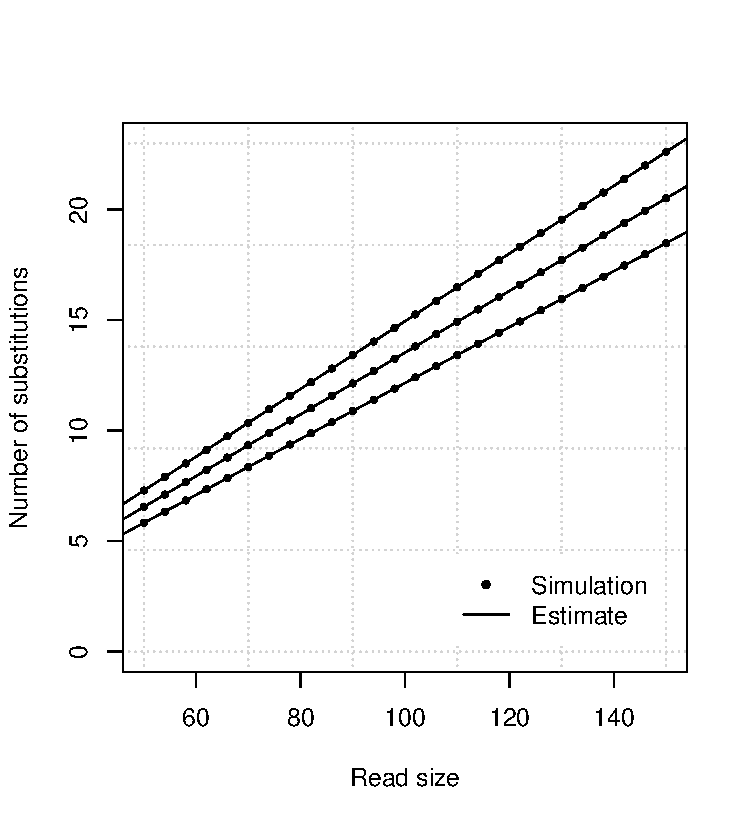
\includegraphics[scale=0.445]{simulp-average.pdf}
\caption{\textbf{Example estimates of average number of deletions}. The
analytic combinatorics estimates of proposition~\ref{th:avsub} are
benchmarked against random simulations.  The average number of
substitutions are shown for seedless reads of given size, either estimated
by 10,000,000 random simulations (dots), or by the method described above
(lines). The curves are drawn for $d=17$, $p=0.08$, $p=0.10$ $p=0.12$
(from top to bottom). The difference never exceeds 0.004 on the examples
shown here.}
\label{fig:simulpdel}
\end{figure}


\subsection{Average size of error-free intervals}
\label{sec:avsz}

Another quantity of interest is the average size of error-free intervals.
for this we need to mark two quantites: the total size of intervals and
the number of intervals. A question we need to decide straight away is
whether an interal of size zero is an interval. We will get two different
answers, depend on whether we answer yes or no to this question.

We start from expression

\begin{equation}
\tag{\ref{eq:altSp}}
(1+F_d(z)) \sum_{n=0}^\infty \big( pz(1+F_d(z)) \big)^n.
\end{equation}

We can label every error-free interval with the variable $u$ by replacing
$F_d(z)$ with $uF_d(z)$. We can also count the cumulative size of
error-free intervals through the variable $v$ by replacing $F_d(z)$ with
$F_d(zv)$. We thus obtain the weighted generating function of three
variables

\begin{equation*}
(1+uF_d(zv)) \sum_{n=0}^\infty \big( pz(1+uF_d(zv)) \big)^n =
\frac{1+uF_d(zv)}{1-pz(1+uF_d(zv))}.
\end{equation*}

From there, we need to derive with respect to $v$ and integrate with
respect to $u$.








%%%%%%%%%%%%%%%%%% Inexact seeding %%%%%%%%%%%%%%%%%%%%%
\section{Inexact seeding}

We now consider a more challenging problem. The ongoing development of
algorithms and data structures makes it possible to search inexact seeds,
\textit{i.e.} sequences that are very similar but not identical to the
target. This comes at greater cost than finding exactly similar sequences,
but it may be worth it because the chances are higher to identify the
target. By tolerating errors in the seed, one can look for longer seeds,
which also reduces the false positive rate.

Before showing how to compute the probabilities that a read contains
an inexact seed, let us roll back to the simplest error model that we have
see so far, namely substitutions only. Figure~\ref{fig:sketchinexact}
illustrates graphically the relationship between intervals, substitutions
and seeds.

\begin{figure}[h]
\centering
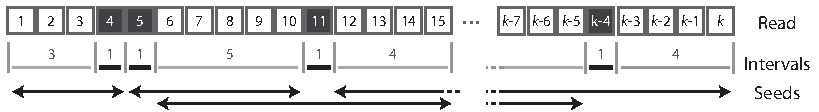
\includegraphics[scale=0.88]{sketch_inexact_seeding.pdf}
\caption{\textbf{Inexact seeding}. Substitutions (black squares) occur
uniformly at random within the read. They delimit error-free intervals.
Inexact seeds (arrows) are the longest stretches of the read that contain
at most one sbustituttion.}
\label{fig:sketchinexact}
\end{figure}


\begin{definition}
\label{def:seed}
An \textbf{inexact $d$-seed} is an interval of size at least $d$ that
contains at most a bustitution and no other error.
\end{definition}

In other words, an inexact seed is either an error-free interval of size
at least $d$, or the concatenation of two error-free intervals and a
substitution, with total size at least $d$. An exact $d$-seed is an
inexact $d$-seed, but the converse is not true. In this section, a
``seedless'' read will designate a read that does not contain any inexact
seed.

As in the case of exact seeding, we will give a construction of seedless
reads, find the corresponding weighted generating function and extract the
asymptotic behavior of the coefficients. Transfer matrices will come in
handy to express the dependence between the error-free intervals on either
side of a substitution. Because the read is seedless, the sum of the sizes
of the intervals on the left hand side and on the right hand side must not
exceed $d-2$ (the substitution adds $1$ to the size of the seed).

In other words, an error-free interval of size $k$ can be followed by an
error-free interval of size $0$, or size $1$, or size $2$, \ldots, or size
$d-k-2$. These intervals have respective weighted generating function $1$,
$qz$, $(qz)^2$, \ldots, $(qz)^{d-k-2}$, so the transfer matrix is

\begin{equation}
M(z) = pz\left[
\begin{matrix}
1 & qz  & (qz)^2 & (qz)^3 & \ldots & (qz)^{d-3} & (qz)^{d-2} \\
1 & qz  & (qz)^2 & (qz)^3 & \ldots & (qz)^{d-3} & 0          \\
1 & qz  & (qz)^2 & (qz)^3 & \ldots & 0          & 0          \\
\vdots & \vdots & \vdots & \vdots & \ddots & \vdots & \vdots \\
1 & qz  & (qz)^2 & 0      & \ldots & 0          & 0          \\
1 & qz  & 0      & 0      & \ldots & 0          & 0          \\
1 & 0   & 0      & 0      & \ldots & 0          & 0
\end{matrix}
\right].
\end{equation}

Note that all the terms are multiplied by $pz$ because we have to prepend
a substitutoin, with weighted generating function $pz$.

Since the sequence may start with an error-only interval of any size from
$0$ to $d-2$, the vector of starting ojects $U(z)$ is $(1, qz, (qz)^2,
\ldots, (qz)^{d-2})$, and because the same holds for the end of the
squence, the vector of end state $V$ is $(1,1, \ldots, 1)^T$.

By proposition~\ref{th:TM2WGF}, the weighted generating function of
seedless reads can be computed as $1+U(z) \cdot (I-M(z))^{-1} \cdot V$.
This expression is not easy to evaluate for large matrices, but it can be
pre-computed for a useful range of values of $d$. The solution can always
be expressed as the ratio of two polynomials, and even though their degree
is high, the asymptotics can be found easily by numerical approaches.

\begin{example}
Let us revisit example~\ref{ex:num1}, where we approximated the
probability that a read of size $k=100$ is seedless for $d=17$ and for a
substitution rate $p=0.1$; but this time we allow the seed to contain one
substitution.  The matrix $M(z)$ is $16\times16$ and the weighted
generating function $1+U(z)\cdot(I-M(z))^{-1}\cdot V$ can be written as
$P(z)/Q(z)$, where $P$ is a polynomial of degree 152 and $Q$ is a
polynomial of degree 153.  Using numerical methods to find the root of $Q$
with smallest modulus, we obtain $z_1 \approx 1.079244$. Likewise,
we obtain $-P(z_1)/Q'(z_1) \approx 2.326700$, so the probability
that the read is seedless is approximately
$2.326700/1.079244^{101} \approx 0.0010511$.
For comparison, a 99\% confidence interval obtained by performing 10
billion random simulations is $0.001049-0.001054$.
% The magic number is 1051660 out of 10 billion.
In these conditions, the chances that the read contains an exact seed is
90.4\%, whereas the chances that it contains a seed with one substitution
is 99.9\%.
\end{example}


\begin{figure}[h]
\centering
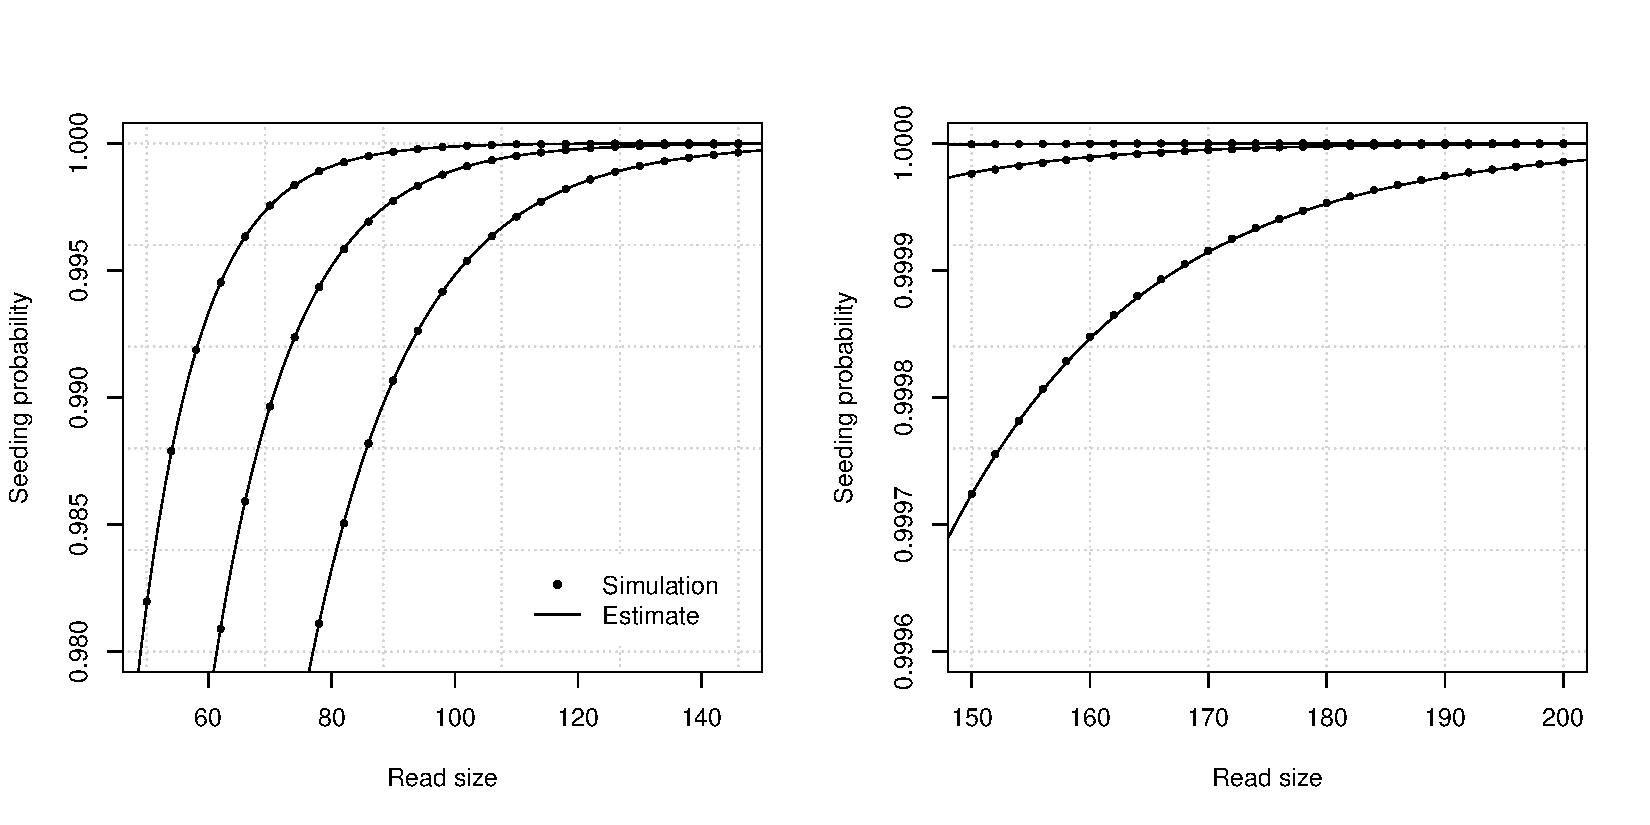
\includegraphics[scale=0.445]{simulp-inexact.pdf}
\label{fig:simulpinexact}
\caption{\textbf{Example estimates for inexact seeding with substitutions
only}. The analytic combinatorics estimates of proposition~\ref{th:pins}
are benchmarked against random simulations.  Shown on both panels are the
probablities that a read of given size contains an inexact seed, either
estimated by random simulations (dots), or by the method described above
(lines). The curves are drawn for $d=17$, $p=0.08$, $p=0.10$ or $p=0.12$
(from top to bottom). 10,000,000 simulations are run on the left panel and
100,000,000 on the right one.  The difference never exceeds 0.0002 on the
examples shown here, which is the expected variation for this number of
random trials.}
\end{figure}












%%%%%%%%%%%%%%%%%% Inexact seeding %%%%%%%%%%%%%%%%%%%%%
\section{Caveats and complements}

\subsection{Low error rates}

In case the error rate is low...

\subsection{Other divergence models}

The difference between the sequences does not have to be sequencing
errors, they can also be evolutionary distances.

\subsection{Inexact seeding with more than one error}

This is fucking impossible...






%%%%%%%%%%%%%%%%%% Inexact seeding %%%%%%%%%%%%%%%%%%%%%
\section{Discussion}

Voila.


%---------------------------------------------------------------
%---------------------------------------------------------------

\bibliography{pubmed,extra}
\bibliographystyle{plain}

%----------------------------------------------------------------

\end{document}

%gs -dNoOutputFonts -sDEVICE=pdfwrite -o out.pdf latex.pdf 
